\documentclass[a4paper, oneside]{discothesis}

% use utf8 instead of latin1 when using LaTeX in windows
\usepackage[latin1]{inputenc}
\usepackage[font={small}]{caption}
\usepackage{subfig}
\usepackage{listings}
\usepackage{url}
\usepackage{wrapfig}
\usepackage{lscape}
\usepackage{rotating}
\usepackage{epstopdf}
\usepackage{float}


%%%%%%%%%%%%%%%%%%%%%%%%%%%%%%%%%%%%%%%%%%%%%%%%%%%%%%%%%%%%%%%%%%%%%%%%%%%%%%%%%%%%%%%%%%%%%%%%%
% DOCUMENT METADATA

\thesistype{Master Thesis}
\title{Towards Datamarkets with Bitcoin}

\author{Francisc Nicolae Bungiu}
\email{fbungiu@student.ethz.ch}
\institute{Distributed Computing Group \\[2pt]
Computer Engineering and Networks Laboratory \\[2pt]
ETH Z�rich}

% You can put in your own logo here "\includegraphics{...}" or just comment the command
% \logo{}

\supervisors{Christian Decker, Dominic W{\"o}rner, Laura Peer\\[2pt] Prof.\ Dr.\ Roger Wattenhofer}

% You can comment the following two commands if you don't need them
% \keywords{Keywords go here.}
% \categories{ACM categories go here.}

\date{\today}

%%%%%%%%%%%%%%%%%%%%%%%%%%%%%%%%%%%%%%%%%%%%%%%%%%%%%%%%%%%%%%%%%%%%%%%%%%%%%%%%%%%%%%%%%%%%%%%%%

\begin{document}

\frontmatter % do not remove this line
\maketitle

\cleardoublepage

\begin{abstract}

\hspace*{12pt} In recent years, there has been a widespread expansion of data collection and complex methods to analyze such 
collected data. Everyone is constantly generating data by using a large range of computers, smartphones, and gadgets.
In addition, there is an emerging trend towards the Internet of Things technologies that consist
of billions of sensor nodes creating massive amounts of data, but with no incentive to share. To provide an incentive for
data sharing, data markets need to be created such that interested customers can subscribe to and 
pay for the acquired data. Bitcoin provides an Internet-native payment mechanism, and protocols on top of Bitcoin are 
able to support small payments and avoid high cumulated transaction processing costs.

	The aim of this thesis is to propose, implement and evaluate a centralized, low-trust and secure scheme 
that allows buyers to purchase data from any Internet-connected sensor node using Bitcoin payments. 
It first examines existing Bitcoin constructs and protocols such as micropayment channels to aggregate 
payments and minimize transaction fees, and contracts between protocol participants to minimize trust. 
In a second stage, these building blocks are combined, and a full two-hop payment protocol is derived. 
Finally, this protocol is implemented and experimental results are charted.

	The results of the evaluation show that the built system is well-suited for the Internet of Things scenario,
allowing buyers to purchase data in real-time. In addition, the evaluation proves that the protocol allows 
human judgment to be taken out of the loop and supports complete automation. 
\end{abstract}

\tableofcontents

\mainmatter % do not remove this line

% Start writing here
\chapter{Introduction}

\hspace*{12pt} The Internet of Things (IoT) is a novel concept that has rapidly expanded in the last few years, 
referring to the network formed by any physical object embedded with sensors and connectivity that enables such 
nodes to exchange data. This network can include objects such as as Radio-Frequency  Identification (RFID) tags, 
sensors, smartphones, etc. The IoT technology allows these objects to be queried for data and controlled 
remotely \cite{iotsurvey}, having a great impact on the every-day life of users, and resulting in 
efficiency and financial benefits.

Sensor nodes with Internet connectivity enable attractive sensing applications in various domains, ranging from
health-care, security and surveillance, event forecasts, environmental monitoring, agriculture automation, 
energy consumption, transportation, etc., creating data markets in which they can actively participate.
However, IoT is still lacking an efficient payment method and is limited by high transaction costs.
\cite{sheng2013sensing} introduces the concept of Sensing as a Service, in which a number of sensors 
offer their generated data as a service to interested entities through a central operator for an agreed cost.

Most existing payment protocols for the Sensing as a Service model involve a third-party to process payments
and arbitrate disputes, which results in higher costs and reduced efficiency. Another approach is to rely on Bitcoin, 
a decentralized electronic payment system. Bitcoin has at its root the block chain, a transaction database 
that is shared by all network nodes. However, the solutions following this approach fail to address the 
scalability problem of Bitcoin: they rely on atomic operations that are completed directly on the block chain, 
thus increasing its size. At the moment, Bitcoin supports less than 7 transactions per second with a 1 megabyte block limit,
with a fee per transaction of $0.0001$ BTC, equivalent to $0.02$ USD. Broadcasting a high volume of small-value transactions 
for each individual data query is clearly not feasible since Bitcoin does not support such a high transaction rate, and 
the associated fees could easily exceed the transfered amount.

This project proposes a centralized, low-trust and secure scheme that allows and incentivizes sensor nodes
to share sensed data and get paid in exchange in bitcoins. The presented solution relies on micropayment 
channels to solve the scalability problem of Bitcoin by bundling several small payments for each set 
of acquired data and only publishing the final, aggregated transaction to the network. 
In order to confer a low-trust relation between the system entities, the protocol relies on contracts 
that pass the payment obligation down from the buyer to the central coordinator, and then to the sensor node. 
In addition to the theoretical model, a proof-of-concept is implemented based on the Android built-in sensors
and evaluated on the Bitcoin TestNet.

\section{Background}

In the following sub-sections, the background on the used concepts and sub-protocols is presented.

\subsection{Bitcoin}

\hspace*{12pt} Since its invention in 2008 \cite{satoshibitcoin}, Bitcoin has grown into a global electronic payment system.
It uses peer-to-peer technology to transfer funds with low transaction fees and no need for a central authority 
such as a financial institution, making it an attractive alternative to traditional payment methods.
A proof-of-work system and cryptographic protocols are the building blocks of the protocol, with peers participating
in the network being responsible for processing transactions and issuing of bitcoins. 

\vspace*{5pt}
\begin{figure}[!ht]
  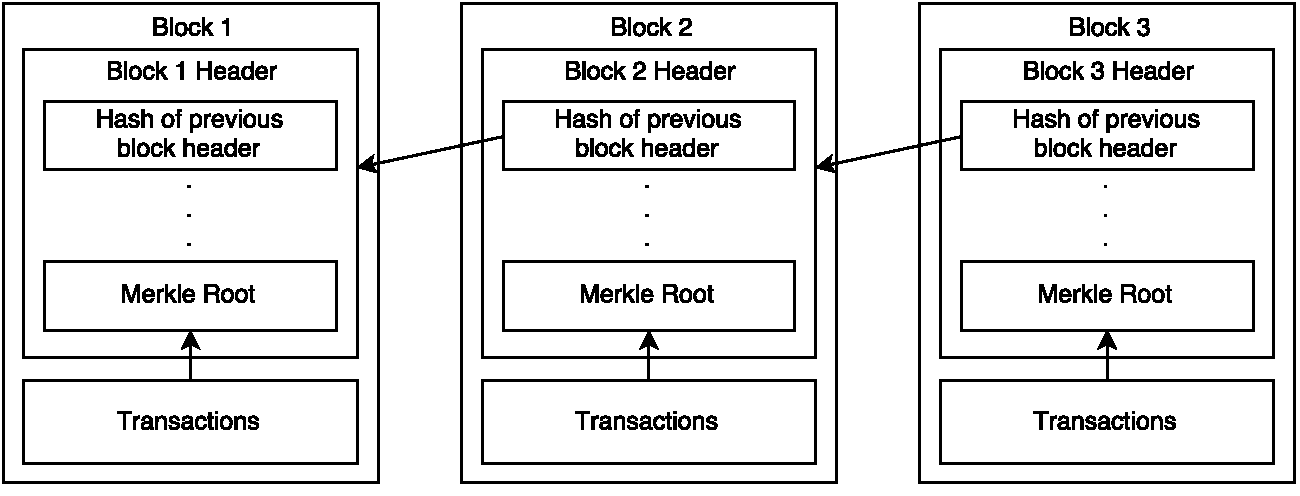
\includegraphics[width=\textwidth]{figures/Blockchain}
  \caption{A simplified representation of the Bitcoin block chain.}
\end{figure}

Bitcoin relies on public key cryptography to authenticate transactions. Each peer in the network has one or more 
public and private key pairs that are stored in a file called a wallet. In order to support and authenticate transactions, 
an address is derived from the public key and disclosed to the participants.
Transactions consist of one or more inputs (references to previous transaction outputs)
assigning the value of all inputs to one or more outputs. An output consists of a tuple of a specified
bitcoin amount, and an output script, called scriptPub. When trying to claim the funds, an entity must
create a signature script (scripSig), which has to satisfy the conditions in the previous output's pubkey scripts.
In most cases, the script only requires a signature matching the address, which proves the possession of the 
corresponding private key. The difference between the total input amount and the total
output amount in a transaction represents the transaction fee.
A peer holding a private key can sign a transaction spending some of its wallet's amount to some other address, and 
any other peer that sees this transaction can verify the signature using the peer's public key. In order to claim an
output, the payee must prove that it possesses the private key corresponding to the public key included as the destination
of the transaction. Thus, the available funds are represented by the amount of all unspent transaction outputs the 
peer possesses a private key for.

In order to be validated and accepted by the peers, 
a transaction needs to be broadcast to the network. Special network nodes, called miners, will then timestamp it by 
applying a hash function into a continuously growing chain of hash-based proof-of-work. 
This forms a record, called the block chain, containing all transactions in Bitcoin ever made, that cannot be 
changed without redoing the successive proof-of-work. The public ledger is distributed to all network peers and 
is crucial for protection against double spending and modification of older transactions. 
The proof-of-work performed in Bitcoin is based on HashCash \cite{hashcash}, which means new blocks containing one or more 
transactions are only accepted into the ledger if the hash of the block header contains a specified number
of zeros as a prefix, adapted dynamically to produce blocks at a constant rate. This means that the expected
time for a transaction to be included in a block, and thus, confirmed, is $10$ minutes. The computation, called mining, 
is incentivized through fees that are earned by the nodes performing it.

\subsection {Micropayment channels}

\hspace*{12pt} Unlike traditional payment methods, Bitcoin transactions are very cheap in terms
of fees, but still have a considerable cost given the mining and storing they require. The context
of Internet of Things requires a high volume of small-value payments, thus the overall fees
might reach and surpass the value of the actual transactions. In addition to this, broadcasting
several transactions to the Bitcoin network in a very short time window will trigger network anti-flooding
algorithms, which will result in either the transactions being delayed or, even worse, not relayed. 
Last, the payee of such small transactions will end up with a wallet full of ``dust'', small outputs
that cost more to be spent than their actual value.

To address these issues, the construct of payment channels was introduced in Bitcoin \cite{hearnmicropay}. 
After an initial setup process between two participants, the payer can start sending tiny payments to the other party
off the block chain at high speed, without paying high transaction fees, in a trust-free manner.

\vspace*{5pt}
\begin{figure}[!ht]
  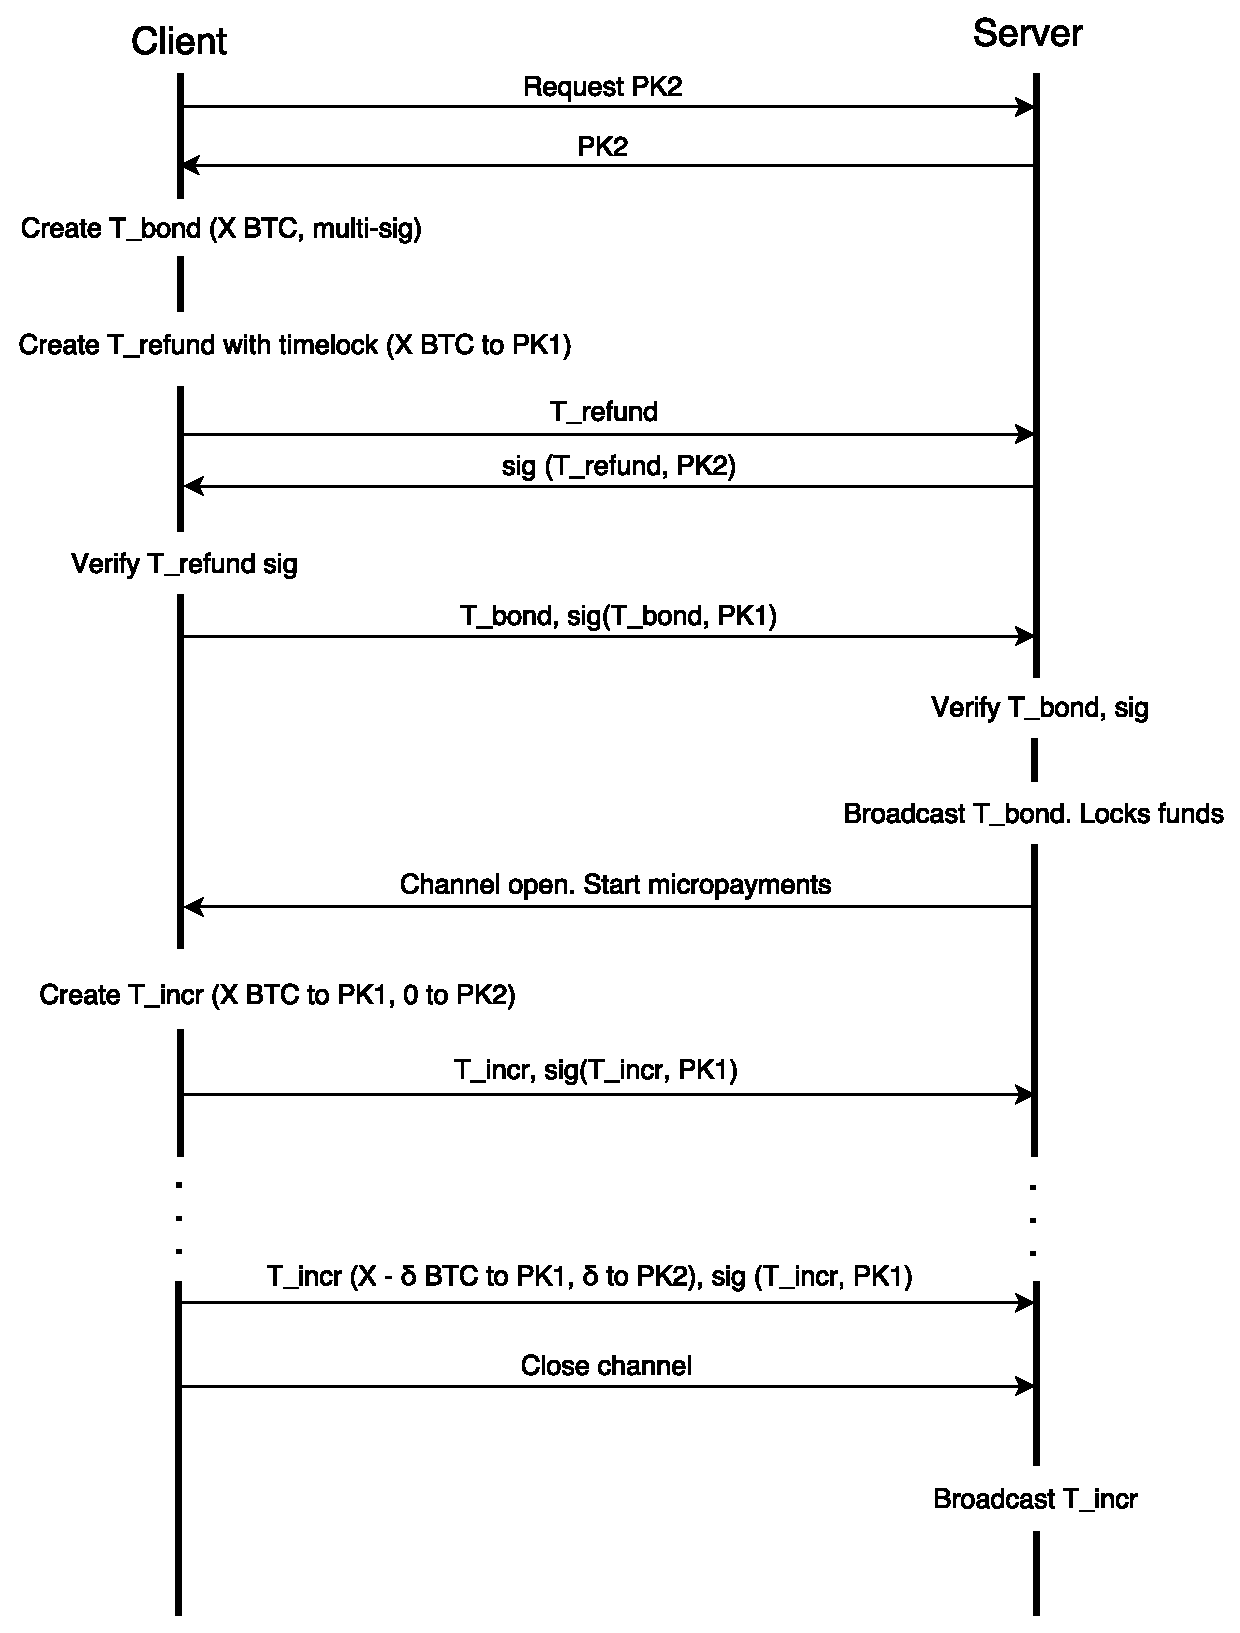
\includegraphics[width=\textwidth]{figures/MicropaymentSeq}
  \caption{Micropayment channel protocol: setting up the shared account (bond transaction), creating the refund 
  transaction, and updating the incremental payment transaction.}
\end{figure}

Consider a client that is interested in a certain service offered by a server.
To benefit from the service, it will pay the server in bitcoins. Since none of the
participants know each other, a zero-trust solution is necessary to reassure both client that it will
not lose its bitcoins in case the server does not provide the data, and that the server will
not provide the promised service without getting remunerated. The construct works in two stages.
First, the client creates a multi-signature transaction, a shared account requiring signatures
of both participants to spend from it, that pre-allocates a certain amount of 
bitcoins for use in the channel. This shared account is called the {\it bond transaction}. 
If the client signs and immediately sends this transaction to the server,
the server could simply broadcast it and keep the money hostage. Thus, the client keeps the bond transaction
private for now and creates another one, called a {\it refund transaction}, and sends it to the server to sign it. 
This transaction refunds the entire value to the client, but it {\it time locked} using the nLockTime feature of Bitcoin,
ensuring it will not become valid until some time in the future (channel lifetime). 
If the server vanishes at any point, the client can then use the refund transaction 
to get all the money back at channel expiration time.

Once the refund has been signed by the server, the client can safely send the signed bond transaction.
After verifying the signature, the server broadcasts it to the network, locking
in the money and opening the channel between the two parties. 

At this point, the work-and-pay cycles can begin. Initially, the client creates a new transaction
spending from the shared account and adds two outputs: one to its own address with the full amount, 
and one to the address of the server. After signing it, the client sends it to the server.
When a new service is requested, the transaction is updated by the client by increasing the
value to the server and decreasing the value allocated to its own address. In each update cycle, the
transaction is signed and handed over to the server. When the time comes and the client wishes
to close the channel, it notifies the server, which in turn signs the transaction with the 
highest value alloted to it and broadcasts it to the network. This step closes the channel, unlocking
the client's remaining money and making the server's money available for spending. The client could be
tempted to broadcast an older transaction that gives less money to the sensor node than it deserved
for services it benefited from, but it is missing the server's signature. Thus, the construct of micropayment
channels prevents misbehavior of both parties.

\subsection{Hashed Time-Lock Contracts (HTLCs)}\label{htlcintro}

\hspace*{12pt} Hashed Time-Lock Contracts, or {\it HTLCs}, are block chain enforced contracts
that require the recipient of a payment to reveal a previously generated secret in order to claim the sent funds.
This construct can be used to provide end-to-end security in multi-hop payments, by preventing the 
intermediaries from delaying or keeping funds for themselves.

To create an HTLC, a special {\it HTLC setup transaction} is created. Its output can only be claimed 
by the final recipient {\it B} of the payment using a previously created secret.
In order to receive a payment, {\it B} has to generate a secret {\it R} and hash it to obtain {\it H}. 
Then {\it H} and B's address are directly transferred to the payer {\it A}. 
At this step, all nodes on the  payment path between the sender {\it A} and the recipient {\it B}
need to create HTLC setup transactions connected to the output of a shared account 
using the provided hash H. The output of the HTLC setup contains a pubScript as shown in
\ref{fig:htlcpubscript}, which requires
a signature from both participants (first branch), or the next hop provides {R'} such that
it hashes to {\it H}. Once all setup transactions are in place, the recipient {\it B}
can release {\it R} to claim the funds from the previous node. The secret is then revealed
step by step by all nodes on path all the way back to {\it A}, which completes the transfer.

\vspace*{5pt}
\begin{figure}[tbp]
  \centering
    \subfloat[HTLC pubScript.]{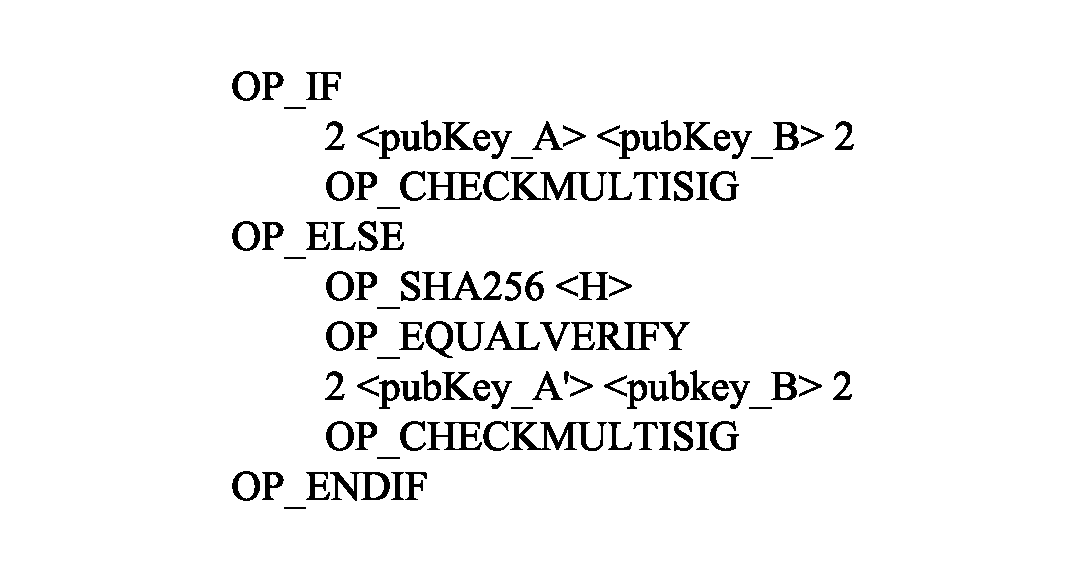
\includegraphics[width=0.5\textwidth]{figures/HTLCPubScript}
    \label{fig:htlcpubscript}}
    \subfloat[HTLC Transaction structure.]{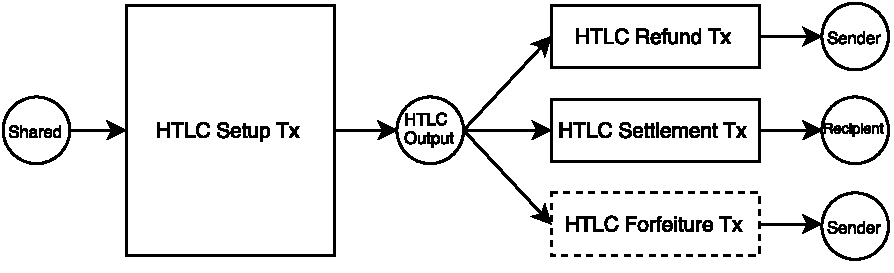
\includegraphics[width=0.5\textwidth]{figures/HTLCTxs}
    \label{fig:htlctxstructure}}
\end{figure}

To prevent the intermediaries from delaying the funds, stealing or keeping them hostage, 
HTLC refund, settlement and sometimes forfeiture transactions are created, all three types
claiming the HTLC output. The detailed structure of these transactions is given in the 
Appendix \ref{fig:pubscripts}.
The {\it HTLC refund transaction} is similar to the refund that is created in the micropayment
channel setup protocol, but has a higher time lock to give the sender enough time
to react, should the receiver not cooperate.
The {\it HTLC settlement transaction} guarantees the receiver it can pull the funds if it 
is in the posession of the secret. It is important for the sender to use different signing keys
{\it A} and {\it A'} for the two branches of the HTLC output. Otherwise, the receiver 
could simply reuse the signature of the settlement transaction in the if-branch and claim
the funds without ever revealing the secret, since the signature is valid for the entire pubScript.
Lastly, the {\it HTLC forfeiture transaction} addresses the case in which the sender and the
receiver agreed to void the HTLC and remove the output. If the receiver comes in possession
of the secret at a later stage, it still has the signed settlement transaction that it 
could simply broadcast and steal the bitcoins. Because of this, every time the receiver
backs off from the HTLC, it creates and hands over a forfeiture transaction that transfers the bitcoins
back to the sender. Should the receiver broadcast an older setup transaction,
the sender can simply use the forfeiture to get the money back.

The main use of the HTLCs is to keep as many transactions as possible off the block chain.
In order for this to work, the recipient, instead of broadcasting the settlement transaction to reveal the 
secret and claim the money, it can simply reveal it directly to the sender. This way, both parties
can agree on removing the HTLC output from the setup transaction, updating the output allocated to the
recipient with the amount of the HTLC. If the recipient chooses to void the HTLC instead, it can
sign a forfeiture transaction and hand it over to the sender, guaranteeing the sender that
it will not use an older setup transaction. By doing this, the HTLC output is again
removed, and its value is added back to the output of the sender.

\section{Related work}

\hspace*{12pt} Following the expansion trend of the Internet of Things technologies, there has been an increasing interest in 
creating secure payment protocols that allow customers to acquire sensor data efficiently. 

\cite{iotzhang} introduces a new low-trust E-business architecture that is tailored 
for IoT. This architecture is based on Bitcoin, eliminating the need for a 
third-party in the process. In order to make a payment and receive the data in exchange, the buyer and the data provider 
make an offer-proposal exchange, then build a transaction that spends the required amount and publish it to the network. 
A similar approach is proposed in \cite{moneyfly}, where the encrypted data is directly included in the 
block chain after a payment is made, which only the buyer in possession of the corresponding private key can decrypt.
In both approaches, all transactions, no matter how small, need to be published to the network, which results in high 
cumulated fees and time-wise inefficiency, thus being directly affected by the scalability problem of Bitcoin.

Work has also been done on micropayment protocols that reduce fee costs.
Amazon Flexible Payment Service uses a central provider that aggregates 
clients' micropayments into macropayments that are flushed to the seller at specific times. This solution
does not provide anonymity, since the central provider can keep track of all payments, and moreover,
was discontinued on June 1, 2015.
Other protocols \cite{microrevisited} involve a probabilistic approach. Using a selection rate {\it s}, it
discards all unselected micropayments and selects one with probability {\it s} that can be deposited for an amount
{\it 1/s} times bigger than the original amount. This should ensure everyone gets, on average, the expected amount. 
However, this solution lacks anonymity, requires PKI certificates and comes closer to a bet than an actual transaction.
The same probabilistic approach is adopted in \cite{micropay2}, but this solution needs a third-party mediator if users
are dishonest.

The \cite{couponbased} paper proposes an anonymous, semi-offline micropayment system for transactions in IoT. 
In this approach, an electronic coin is obtained by iteratively applying a hash function to some initial seed, 
thus allowing the user to spend it in fractions, by presenting a set of hash chain nodes to the vendor. 
The protocol is designed to meet the needs of IoT transactions, however, it has limited potential to be 
implemented because it does not rely on an existing payment infrastructure. 
Another coupon-based system has been proposed by Rivest in \cite{Rivest:1996:PMT:647214.720369} and was 
improved by Payeras-Capella (\cite{Payeras-Capella:2003:EAS:1758260.1758276}) to integrate anonymity and 
prevent users from exceeding their account limit. The drawback of the latter is that the financial institution 
needs to be contacted directly before each payment, and any unspent value is lost
in favor of the financial institution. Wilusz \cite{3279} solves these issues by requiring a single 
contact with the financial institution at coin issue time and allowing the user to use unspent fractions in 
future transactions. However, a clearing house is necessary to lock in the coin by the vendor, which 
increases transactions costs, and poses the risk of locking the coin indefinitely.

It is worth mentioning that there have been several proposals and ideas that can be exploited to support
trustless, instant, off-the-chain Bitcoin payments on the Bitcoin discussion forum \cite{forum} by Mike Hearn, 
Alex Akselrod, C.J. Plooy, Tier Nolan etc.

On the Contracts page of the Bitcoin Wiki \cite{hearnmicropay}, Mike Hearn describes an idea
on how to trade with somebody with no trust involved, based on multi-signature transactions. 
Hearn also proposed the idea of trading across multiple currencies without a third party, 
and Tier Nolan formalized it in a protocol that allows the exchange atomically, using time locks and hash commits.

C.J. Plooy presented a draft that combines Bitcoin and Ripple to create a high-speed, scalable, anonymous, 
decentralized, low-trust payment network \cite{ripplebitcoin}. Ripple \cite{ripple} is a real-time gross settlement system
based on a distributed consensus ledger. It manages transactions as as debts between trusted parties. 
In this Bitcoin-specialized variation of the Ripple system, neighboring pairs have a shared account that is 
partly allocated to one of them, and the rest to the other, as agreed between the two, which lowers the 
needed trust. Using sequence numbers to update this transaction as payments in the network are made and 
lock times to prevent blocking the money indefinitely. 

Alex Akselrod proposed \cite{draft} \cite{eschaton} and built a proof-of-concept
for chained micropayment channels with two-phase commits. The original micropayment channel payment scheme was modified
to allow sending funds both ways using commit hashes and cycles of refund transaction updates with decreasing
time locks. However, the proposal suffers from the Bitcoin malleability issue \cite{malleability} 
and the possibility of getting money locked in indefinitely, should the contract transaction be broadcast before 
refund transactions are fully signed.

Peter Todd's proposal in \cite{hubandspoke} provides an efficient way for establishing micropayment
channels between peers with a central hub. This central entity plays the role of a router, forwarding
payments from the payer to the payee. Suppose Alice and Bob have previously established micropayment channels with
the hub. If Alice wishes to send bitcoins to Bob, she should normally establish a new micropayment channel with him.
However, both of them have channels opened with the hub, so Alice can send the funds to the hub, and the hub can then
forward the payment to Bob. Using Hub-and-Spoke payments, payments between buyers and service providers with a central
coordinator can be made efficiently, saving costs in terms of fees. Nonetheless, the forwarding process should be enforced
and secured, part that is noted in the proposal, but without specifying an actual way to do so. 

The Lightning paper \cite{lightning} presents a promising solution to Bitcoin's scalability problem and provides a way to
securely forward payments on a path of peers through block chain enforced contracts. 
It solves the issue by using timelocks on a network of bidirectional micropayment channels combined with 
Hashed Timelock Contracts (HTLC) introduced in Section \ref{htlcintro}. With the introduction of a 
new sighash type which solves malleability, the proposed protocol allows offchain transactions between 
untrusted parties with fully enforceable contracts. However, the IoT scenario requires asymmetrical payments,
from buyers to data providers. Consequently, this solution allowing bidirectional fund transfers cannot be applied to it.

\chapter{Design}

\section{Requirements}

\hspace*{12pt} For the presented use case, a scheme that enables sensor nodes in an Internet-of-Things network 
to share sensed data and get paid in exchange must meet the following requirements:
\begin{itemize}
 \item Provide an entity that the node can register sensor type availability to.
 \item Provide an entity that buyers can query for available data and that can provide sensor node contact
 information.
 \item Scalability: avoid broadcasting all micro-transactions to the block chain.
 \item Efficiency: fast communication between components, payments and data should be confirmed and 
 received instantly.
 \item End-to-end security of the payments: intermediary nodes should not be able to keep funds for themselves.
 \item Anonymous: linking of buyers and sellers and identification across sessions should not be possible.
\end{itemize}

\section{System Overview}

\hspace*{12pt} The design of the payment system achieving the requirements above comprises three major components:
sensor nodes, a central hub, and data buyers. The first component consists of several sensor data providers: 
IoT sensor nodes, Android phones running specialized apps, etc. The central hub plays an essential role 
in sensor node discovery, payment and data relaying. Last, the buyers' component consists of all entities
interested in the sensed data. All three components needs Internet connectivity to communicate with
each other and the Bitcoin network.

\begin{figure}[!ht]
  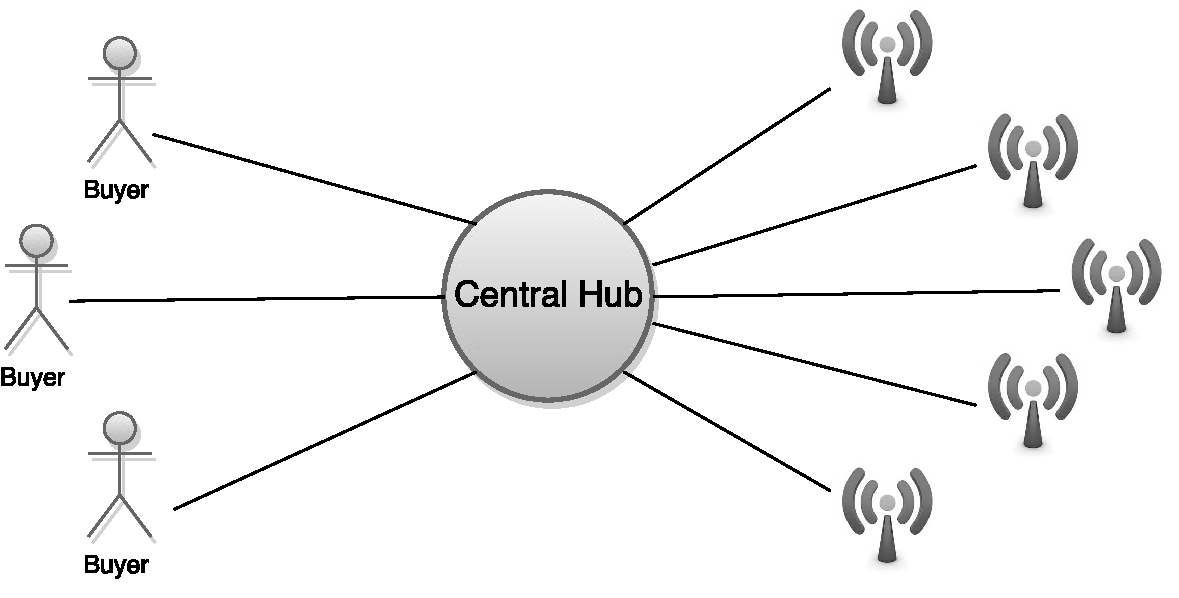
\includegraphics[width=\textwidth]{figures/SystemOverview}
  \caption{System overview: buyers, central hub, and sensor nodes.}
\end{figure}

\section{System components}

\subsection{Sensor nodes}

\hspace*{12pt} The sensor nodes are the data generating elements in the system. Their role is to obtain various
parameters about the surrounding environment and provide this data to interested entities for a fixed price.

In order to participate in the system, the sensor nodes need Internet connectivity to establish 
TCP connections to the central hub. The node then initiates the establishment of a long-term micropayment channel,
for example, $30$ days. Once the setup is complete, the availability of the sensors is signaled to the hub, 
which registers them accordingly for future buyer queries.

\subsection{Buyers}

\hspace*{12pt} This component consists of a simple interface connecting to the hub through a TCP connection. First,
a micropayment channel is established with the central hub. After this initial step, the buyer
can run queries such as:
\begin{itemize}
 \item Node statistics: offer information on the number of connected sensor nodes. 
 \item Sensor statistics: offer information on the types of sensors that are available for purchasing.
 \item Select queries: allow buyers to query for a certain type of sensor data and inform them
 on nodes this data is available on, together with pricing information.
 \item Buy queries: allow buyers to purchase a set of data for a certain sensor type from a selected node.
 This query will return the asked data set.
\end{itemize}

\subsection{Central Hub}

\hspace*{12pt} At the heart of the system lies the central hub. According to the requirements, the hub acts as 
a coordinator, payment forwarding medium and meeting point between the buyers and the data providers. 
It establishes micropayment channels with all sensor nodes and all buyers. On the other hand, each of the 
other two components only need to keep one micropayment channel open, with the central hub.

When a new data provider connects to the central entity, it establishes a TCP connection and sets up a new 
micropayment channel between the two. That is, the hub has to lock in a certain amount for a longer time interval 
({\it 30} days, for example). Assuming numerous data providers, the hub is required to have a high amount of bitcoins
to pre-allocate in each established channel to run the entire system.

To support the two types of connection, the hub is running two servers, 
providing specialized handlers that communicate with each sensor node and buyer connecting to it. 
A driver component coordinates the two subcomponents, book-keeping connected nodes and buyers, and forwards messages
between the buyers and nodes.

\section {Achieving the requirements}

\subsection{Achieving Scalability and Efficiency}

\hspace*{12pt} In order to achieve scalability and efficiency, there are three important factors that need to be taken
into account: the inherent scalability issue of Bitcoin, the number of peer pairs that need
to interact to successfully get payments from buyers to the sensors, and the long and probabilistic 
confirmation times of Bitcoin transactions.

Creating new transactions for each small-value payment would have a very high overhead in terms of fees, 
which reduces the incentive for both the buyers and the sensor nodes to participate in the protocol. 
A high volume of transactions would also delay the transactions being confirmed on the Bitcoin network. 
To address these issues, the proposed system will rely on the previously introduced micropayment channels. 
This mechanism will allow, after a preliminary setup between the parts that wish to transact,
to instantly send small amounts of bitcoins off the block chain, bundling and publishing them to the
network only at the end of a specified time window. Thus, both scalability of Bitcoin and efficiency
of payments are achieved.

One issue that comes with using micropayment channels in the proposed context 
is that its set-up phase takes a considerable time, approximately 10 minutes, until the bond transaction
is confirmed by the network. Thus, setting up a channel between all buyers and nodes becomes 
very inefficient time-wise and causes a lot of overhead on the network since all connections need
to be maintained for the lifetime of the channel.
On the other hand, if the buyers and the sensors have previously established a channel with a central 
entity as in the hub-and-spoke model \cite{hubandspoke}, each will have a single set-up to wait for 
and a single channel connection to maintain.

Last, adding a single central entity may affect the scalability of the system when the number of 
data providers and buyers increases, becoming a performance bottleneck. 
However, the concept of a central hub should be rather treated as a central cloud, which can contain 
several machines maintaining the connections, channels, available sensor data, and load balancers 
that distributed the work across the available machines.

\subsection{Achieving Security}

\hspace*{12pt} To achieve efficient end-to-end security on the path between the buyers and the data providers, 
pre-established micropayment channels are combined with HTLCs. This ensures that
all nodes on the payment path receive their funds and no coins can be gained by defecting.
The method is first presented for neighboring nodes, then extended for full paths.

\vspace*{5pt}
\begin{figure}[!ht]
  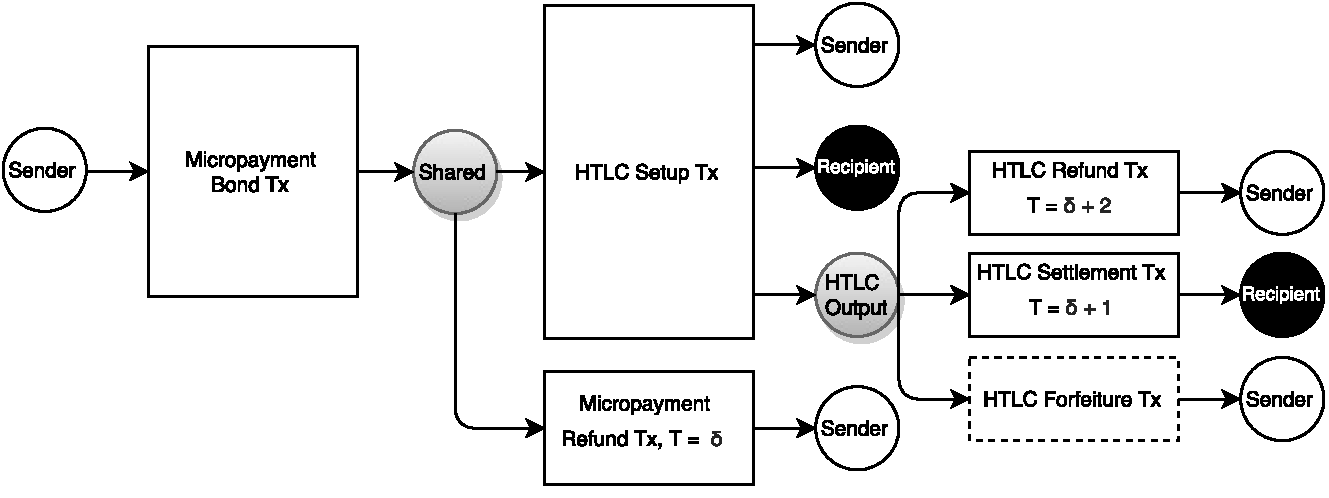
\includegraphics[width=\textwidth]{figures/MicroHTLC}
  \caption{Micropayment channels with HTLCs for end-to-end security on payment paths}
\end{figure}

\hspace*{12pt} First, the two neighboring nodes have to set up a shared account 
(multi-signature output) between the two of them. Once the bond
transaction with the multi-signature output is broadcast to the network, 
the funds are locked in and the micropayment channel is opened. Initially, an HTLC setup 
transaction spending the shared output is created, allocating 
the full channel amount to the sender, and $0$ to the recipient. When a new payment is created,
instead of directly increasing the amount which the recipient, an HTLC output with the
payment amount is added to the HTLC setup transaction, which requires a secret $R$, 
known only by the recipient, to be revealed in order to claim the payment. 
As previously explained in Section \ref{htlcintro}, the HTLC output is spent by three
transactions: the HTLC refund, settlement and forfeiture transactions.  These transactions
are only to be used for conflict resolution.

In a successful collaboration between the two nodes, the recipient will release the secret
to the sender. At this stage, an updated HTLC setup transaction is created, with the HTLC output's value
added to the receiver's output. Should the recipient not be able to reveal $R$, it can also choose to void
the HTLC output, cancelling the transfer and returning the HTLC output's value to the sender's output of the
HTLC setup transaction. The recipient also hands over a forfeiture transaction that guarantees it will
not use an older HTLC setup transaction version, should it receive the secret at a later time.
Multiple HTLC outputs can be active at the same time and new payments can be made without 
any transaction being broadcast to the network.

If the sender does not collaborate to update the HTLC setup transaction, the receiving party has 
to broadcast the most recent HTLC setup transaction before the channel refund transaction 
becomes valid at time $T = \delta$. If the sender still tries to broadcast the channel 
refund transaction, it would be rejected since it double-spends the multi-signature output of 
the bond transaction. Once the HTLC setup transaction is confirmed by the network, the remaining
HTLC outputs become available for spending. If the recipient has the secret, it has time 
until $ T = \delta + 1$ to commit the settlement transaction. On the other hand, if the sender
cannot produce $R$ by time $T = \delta + 2$, the sender will get its funds back 
using the HTLC refund transaction. Should the receiver broadcast an older HTLC setup transaction
with HTLC outputs that it agreed to void, the sender can broadcast the previously received forfeiture
transactions to immediately claim those outputs. Last, if the receiver party vanishes at any point
before broadcasting the HTLC setup transaction, the sender can simply use the channel refund 
transaction to get a full refund of the money it locked into the channel.

\hspace*{12pt} To achieve end-to-end security on the full path between the buyers, central hub, 
and sensor nodes, the protocol above is extended. First, the buyer and the sensor node 
have to establish micropayment channels with the central hub. In order to make a payment, 
the buyer has to first make a request to the final recipient, the sensor node, through the hub, 
which generates a secret $R$, hashes it to obtain $H$, and sends $H$ back to the buyer. 
Using the received hash, the buyer opens a new HTLC flow with the central hub, by adding an 
HTLC output to the setup transaction spending from the shared account between the two. 
Once the process is complete, the hub then uses $H$ to open a corresponding HTLC flow with 
the sensor node. After this step, the sensor can release the secret to the hub to claim its money.
The hub can then use it to claim the funds from the buyer, closing the two HTLCs. This process
provides end-to-end security on the payment path.

\vspace*{5pt}
\begin{figure}[!ht]
  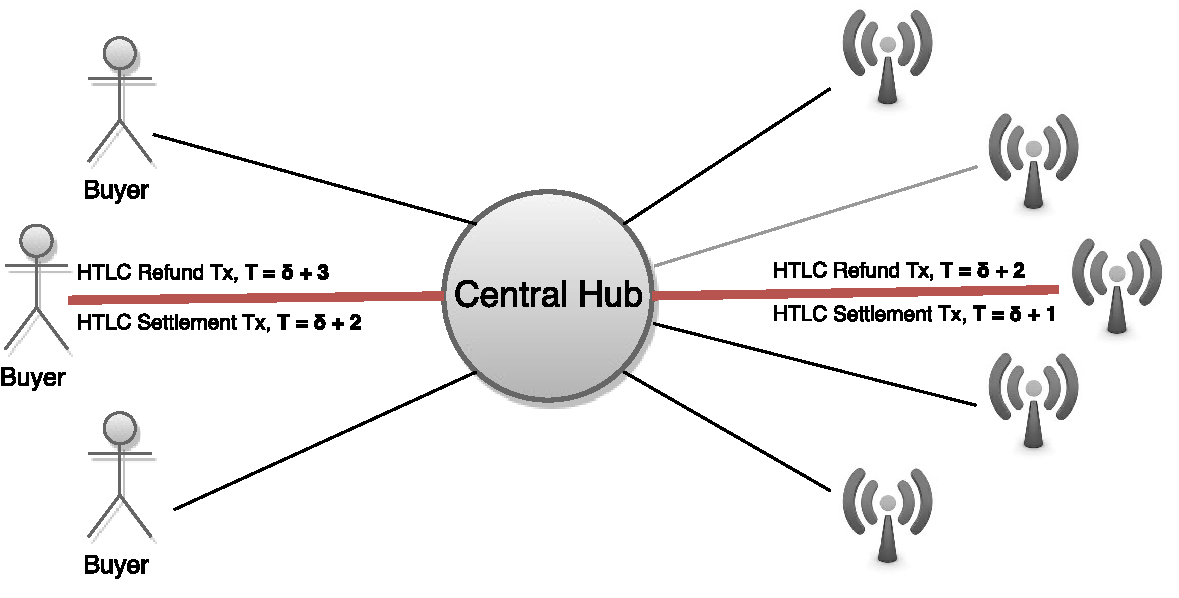
\includegraphics[width=\textwidth]{figures/FullMicroHTLC}
  \caption{Securing payment paths between buyer, hub, and sensor nodes with micropayment channels and 
  HTLCs}
  \label{fig:fullmicrohtlc}
\end{figure}

In order for the protocol to be fully secure in this two-hop payment scenario, the time locks of 
the HTLC refund and settlement transactions from the recipient up to the buyer need to be higher
than the ones from the previous hop (see \ref{fig:fullmicrohtlc}), such that no participant
can reveal the secret so late the upstream is not given the opportunity to claim its coins in time.

\subsection{Achieving Anonymity}

\hspace*{12pt} By design, the role of the central hub is to connect data buyers and sellers, and given that
the lifetime of the established micropayment channels are rather long, the hub can easily analyze
the data a buyer is interested in, build a profile and ultimately, identify it. To address
this privacy issue, buyers could make use of an anonymization network, such as Tor \cite{tor},
open several, shorter-lived sessions, over several vantage points, 
and spread payments and data exchanges on these session when buying different sets of data. 
An additional precaution is to never reuse addresses across sessions. 
This way, profiling becomes more difficult,
and the hub cannot link anymore buyers and data they have purchased through the system.

\chapter{Implementation}

\hspace*{12pt} Following the introduced design, the Java implementation of a proof-of-concept based on 
the Android built-in sensor is presented in this chapter.

\section {API design}

\hspace*{12pt} The implementation of the system is based on {\it bitcoinj}, a Java library that allows users
to work with the Bitcoin protocol. Its features include maintaining a Bitcoin wallet, creating, sending and
receiving transactions, but also more advance constructs such as contracts and micropayment channels. 

From a high-level point of view, the system is designed according to the client-server architecture, 
in which each component is either a client or a server. The buyer component and the sensor subcomponent of the hub 
that are spending funds in exchange for a service are considered clients. On the other hand, the buyer subcomponent 
of the hub and the sensor node component providing data in exchange for bitcoins are considered servers. 

\vspace*{5pt}
\begin{figure}[!ht]
  \centering
  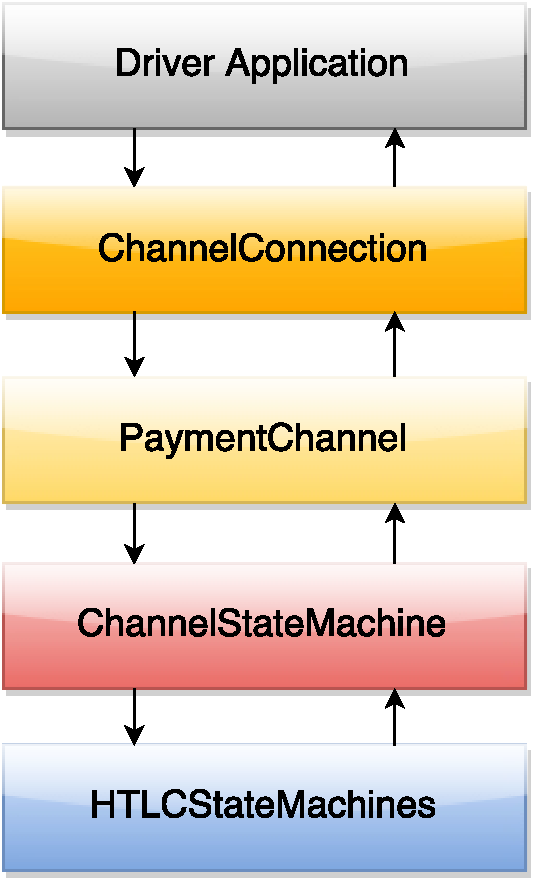
\includegraphics[width=4cm, height=7cm]{figures/LayeredAPI}
  \caption{Five-layered application architecture}
  \label{fig:layeredapi}
\end{figure}

From a logical point of view, each application relies on a layered design, which improves maintainability 
(easy to modify, test, debug, reuse layers), and performance. Layers exchange information through strict interaction.
This approach offers a rigorous separation of concerns and ensures that each layer only interacts 
with the one directly below. Each application is layered according to Figure \ref{fig:layeredapi}:
\begin{itemize}
  \item \textbf{Driver application layer.} This is the topmost layer representing an interface the users can directly
  make use of to access the functionality provided by the lower layers. Following the design patterns from 
  the {\it bitcoinj} library, the ListenableFuture class from the Google Guava library is used to register callbacks 
  in the Driver layer, so the application gets notified once a computation is complete.
  \item \textbf{Channel Connection layer.} This layer is responsible for reading and writing objects to the network.
  The functionality is provided by the {\it niowrapper} package of the {\it bitcoinj} library, which relies on 
  Java NIO: nonblocking, socket I/O. It also provides multiplexing, a technique used to monitor
  multiple I/O operations executing concurrently from a single thread, obtaining high performance and low latency.
  \item \textbf{PaymentChannel layer.} The middle layer is responsible for processing the messages that are received
  through the wire from the layer above, dispatching tasks to lower layer accordingly, receiving results from them,
  and finally constructing message replies and sending them to the connection layer. Simple micropayment channels are
  fully supported by the {\it bitcoinj} library; however, for this project, the package was rewritten to support
  HTLCs and simplified by removing the layer responsible for resuming channels in case of connection failure.
  \item \textbf{ChannelStateMachine layer.} This layer provides a state machine independent of any network protocol.
  It is the Bitcoin-aware layer: it constructs transactions, signs them, schedules refunds for future broadcasts
  to initiate, use, and safely close a micropayment channel.
  \item \textbf{HTLCStateMachines layer.} This layer provides one or more state machines that are responsible 
  for keeping track of the HTLC flow. By allowing several instances to run at the same time, concurrent payments
  are possible.
\end{itemize}

Both clients and servers adhere to the architecture above, with differences in functionality.
In the next subsection, the two component types are introduced in more detail. Their interaction
to run the proposed payment protocol is then described.

\subsection {Client}\label{client}

\hspace*{12pt} The client component represents the payment sender party in the protocol. The responsibilities
of each layer in this component are described in a top-down manner.

At the driver application layer, the client initiates and maintains a connection to the Bitcoin network,
synchronizing and keeping the local block chain up to date. It also loads the wallet of the client,
and establishes a TCP connection to the server it will send payments to. Once the connection with the server is set up,
the micropayment channel establishment protocol is run.

The second layer handles the TCP connectivity. It also acts as a binder between the upper and lower layers
and passes messages received from the server to the PaymentChannel layer. The PaymentChannel layer analyzes
all incoming messages and triggers specific processes and transitions in lower layers, ultimately constructing
appropriate replies that are sent back to the server. 

The client uses the ChannelStateMachine layer to store the progress of establishing a micropayment channel
so it is always in a secure state. Once the channel is successfully opened, the client can start making 
HTLC payments. The states of the HTLC payments are stored at the lowest level, in the HTLCStateMachines layer.
A full client class diagram can be found in the Appendix, Figure \ref{fig:clientuml}.

\subsection {Server}\label{server}

\hspace*{12pt} The server component represents the payment receiver party in the protocol. The responsibilities
of each layer in this component are described in a top-down manner.

At the driver application layer, the server first connects to the Bitcoin network and synchronizes its local
block chain. After syncing the block chain, it starts listening for incoming connections from clients
in the second layer.

When a new client initiates a TCP connection, the server dispatches a handler that runs the micropayment channel
establishment protocol with the client. All messages are processed in the PaymentChannel layer and the state
of the payment channel is stored in the ChannelStateMachine layer. Once the channel between the client
and the server was established, the server can receive payments from the connected client. The states
of the HTLC payments are stored in the HTLCStateMachines layer. A full server class diagram can be found in the
Appendix, Figure \ref{fig:serveruml}.

\subsection {Cross-component communication}

\hspace*{12pt} System components communicate through TCP connections, transmitting Protocol Buffers (protobuf), 
an extensible, efficient, automated, serialization method introduced by Google in 2008. 
After defining the structure of the data that needs to be serialized through an interface description language, 
a compiler generates source code that allows to write and read the data to in a language independent manner.

To support the proposed payment protocol, the needed data structures were defined using protocol buffer message types
in {\it .proto} files. Each such message contains a series of name-value pairs, associating scalar data types 
with field names. Additionally, each field has an integer field that uniquely identifies it. 
The description language also allows specifying field rules:
\begin{itemize}
 \item {\it optional}: a message containing a field with this rule can contain this field zero zero or one time.
 \item {\it required}: a message containing a field with this rule must contain this field exactly one time.
 \item {\it repeated}: a message containing a field with this rule can contain the field multiple times (including zero).
\end{itemize}

Following the pattern endorsed in the {\it bitcoinj} library, messages are extended to support
the communication in the proposed protocol. A full definition of the used protobuf messages can be found
in Appendix \ref{protobuf}. The next subsections will detail out the use of each message in the 
micropayment channel setup and HTLC payments.

\subsection {Establishing a micropayment channel} \label{establishmicro}

\hspace*{12pt} Once the TCP connection between the client and the server components is established, 
the client will initiate the process to establish a micropayment channel between the two. 
The exchange of messages in this sub-protocol is asynchronous to increase throughput and response time.

\begin{figure}[h]
  \centerline{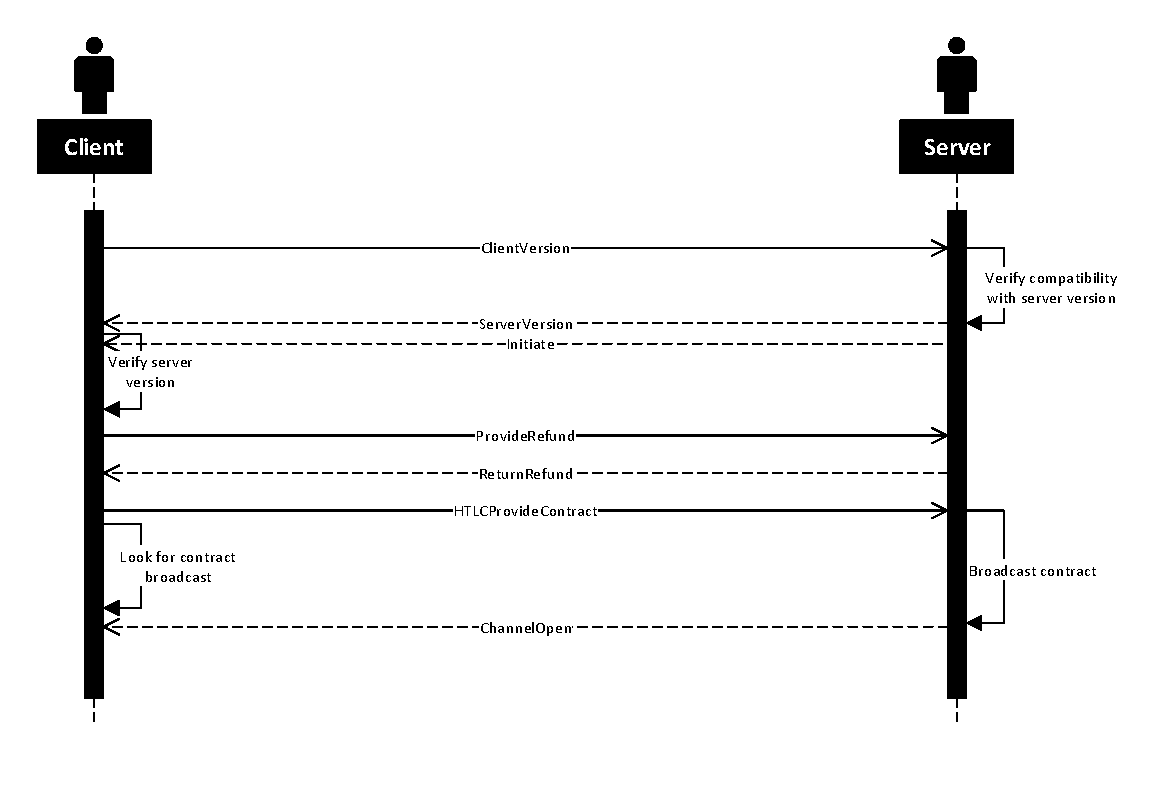
\includegraphics[width=\textwidth]{figures/MicroSeq}}
  \caption{Micropayment channel sequence diagram.}
  \label{fig:microseq}
\end{figure}
\begin{figure}[h]
  \centerline{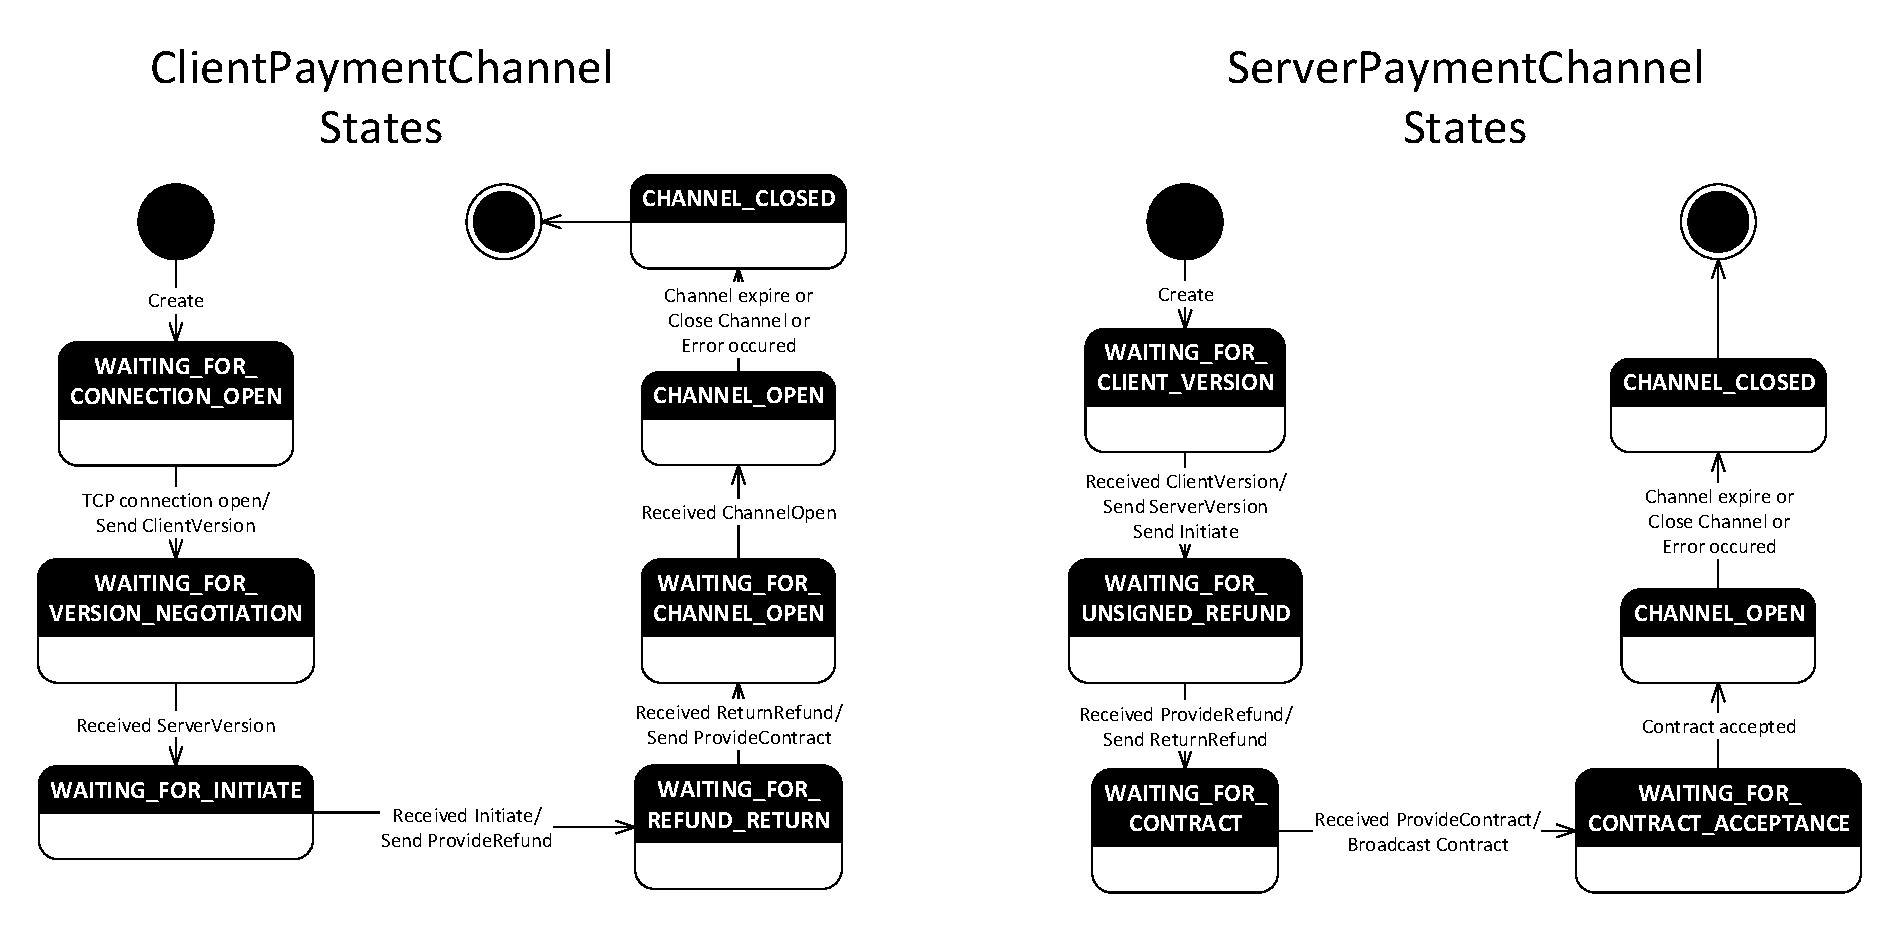
\includegraphics[width=\textwidth]{figures/MicroStates}}
  \caption{Micropayment channel state machine diagram.}
  \label{fig:microstates}
\end{figure}

Figure \ref{fig:microseq} shows the steps and exchange of messages between the client and the server to successfully
set up a payment channel. The logical states of the channel establishment are displayed in 
Figure \ref{fig:microstates}. The transitions correspond to receiving specific messages from the other protocol 
participant. First, the client sends over a ClientVersion message, containing the version of the 
{\it bitcoinj} library it is using, and the time window in seconds the channel should be opened for. The server verifies
if the client version matches its own version, and replies with a ServerVersion message. At this time, the server
also sends the client an Initiate message containing its public key, the expire time of the channel, the minimum
value that needs to be locked into a channel, and the amount of money that the server needs in the initial payment 
for the channel to be opened. The last entry ensures that the client does not open a channel that cannot be 
settled because the server received an amount under the dust is an amount that is below the limits for a 
legitimate transaction.

When the client receives the Initiate message, it checks that its wallet contains enough funds to open the channel
under the requirements imposed by the server, and stores the progress of the channel establishment. The client then
creates the bond and the refund transactions. A ProvideRefund message containing the refund transaction 
and the public key of the client is sent to the server. At this point, the server also stores the progress
the channel setup, signs the received refund transaction and returns it to the client in ReturnRefund.

Once it has received the signed refund transaction, the client checks the signature of the server. After
validating it, the refund transaction is stored and scheduled for broadcast at the time the channel expires.
The client then creates an initial signed HTLC setup transaction spending from the contract transaction 
a minimum value required by the server, and sends both signed transactions to the server in a HTLCProvideContract
message.

At this point, the server checks the signatures of the client and that the HTLC setup transaction indeed correctly
spends from the contract. After validation, the contract is broadcast to the Bitcoin network.
Once the contract is accepted by the network, the funds of the client are locked in, and the server signals 
the client that the channel is open for payments through a ChannelOpen message.

\subsection {Making an HTLC payment} \label{establishhtlc}

\hspace*{12pt} After a micropayment channel is successfully set up between the client and the server,
the client can begin making payments in exchange for data. When it comes to payments, cross-component communication 
is no longer done asynchronously, but synchronously, using batched update rounds. This solution has been chosen 
to support concurrent payments and is needed so that the HTLC setup transaction is always in a secure and 
consistent state on both the client and server side. Otherwise, updates from both sides could be crossing each other 
and invalidate the signatures of the HTLC refund, settlement, and forfeiture transactions attached to the 
HTLC outputs of the setup transaction.

\subsubsection{Batching and round negotiation}

\hspace*{12pt} Figure \ref{fig:roundneg} shows how update rounds are negotiated between the client and server. 
On the client side, updates are always new payments coming in. On the server side, updates can be of two types:
the server is either claiming an HTLC output by revealing the corresponding secret, or wishes to void an HTLC output.
Both protocol participants buffer update requests in a blocking queue while an update round is active.

\begin{figure}[ht!]
  \centerline{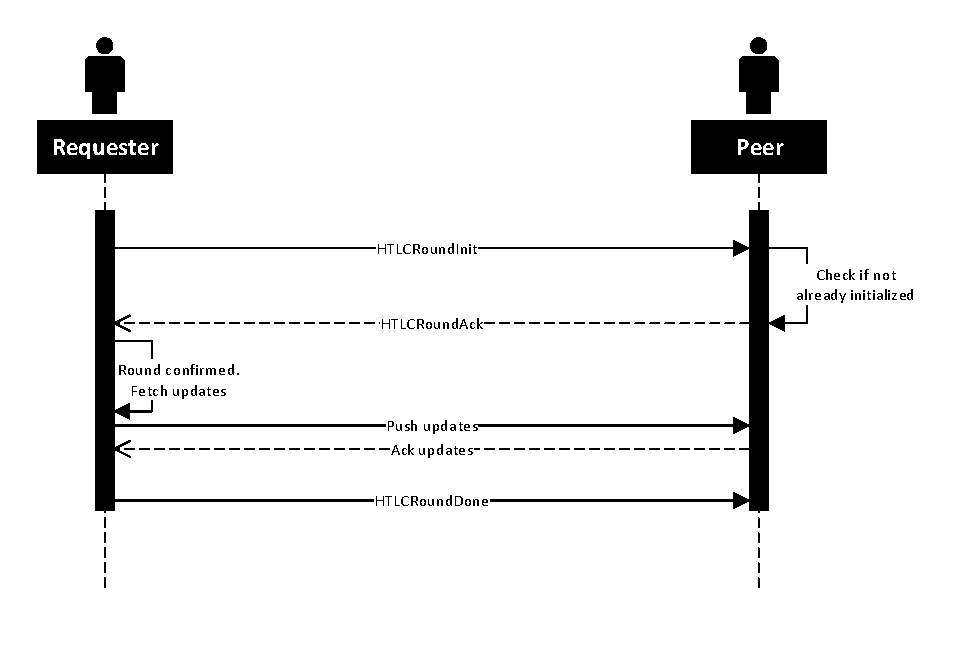
\includegraphics[width=\textwidth]{figures/RoundNegotiation}}
  \caption{HTLC update round negotiation}
  \label{fig:roundneg}
\end{figure}

When one of the components has a new update to push to its peer, it first sends an HTLCRoundInit message to the other
participant. Then, the peer checks if no other update round has been already initialized. If this is the case,
an HTLCRoundAck is sent to the initiator, which confirms the updates can be pushed. In case both participants are
waiting for an HTLCRoundAck message, priority is given to the server. Once the initiator 
finished pushing all updates to the other participant, it marks the end of the round with an HTLCRoundDone message.
If the other participant has buffered updates at this point, it can now safely initiate its own update round.

\subsubsection{Initiating a payment} \label{initpay}

\hspace*{12pt} After the client has secured an update round through the negotiation mechanism presented above, 
it can send new payments to the server. The full process is shown in Figure \ref{fig:htlcsetupseq}. 
The logical states of the payment setup and clearing are displayed in Figure \ref{fig:htlcstates}. 
The transitions correspond to receiving specific messages from the other protocol participant.

\begin{figure}[ht!]
  \centerline{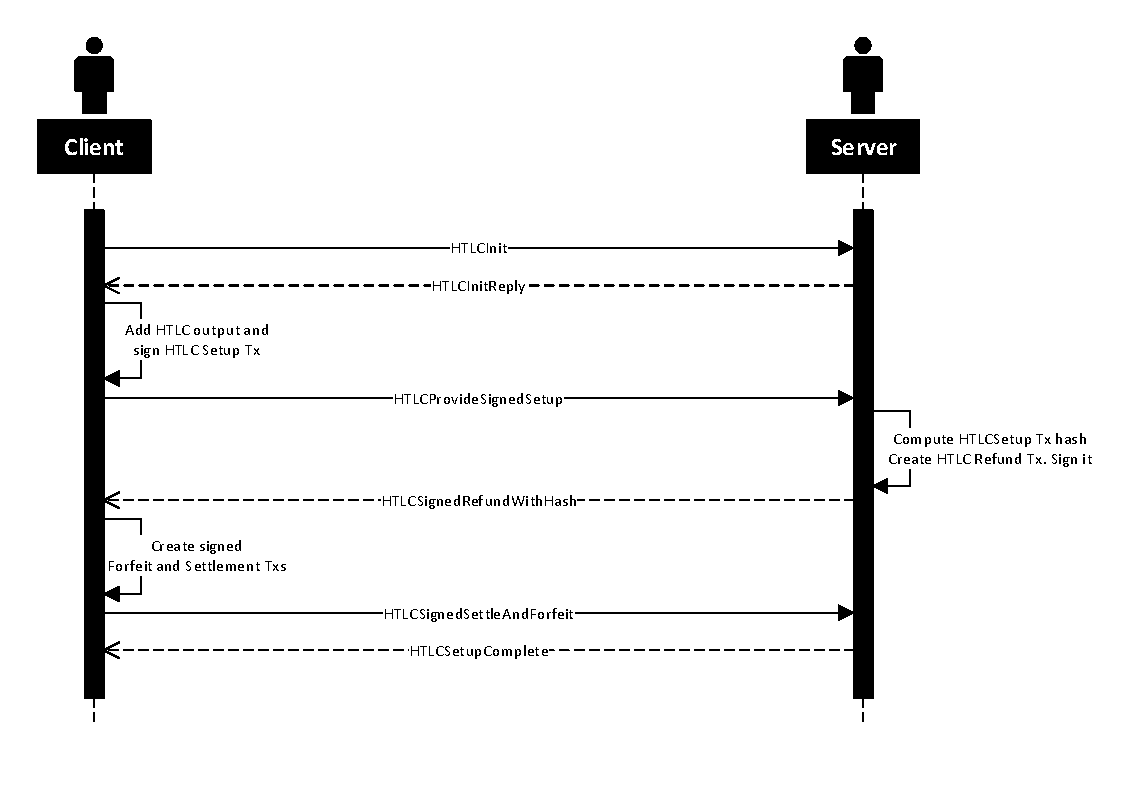
\includegraphics[width=\textwidth]{figures/HTLCSetupSeq}}
  \caption{HTLC Setup sequence diagram}
  \label{fig:htlcsetupseq}
\end{figure}

\begin{figure}[ht!]
  \centerline{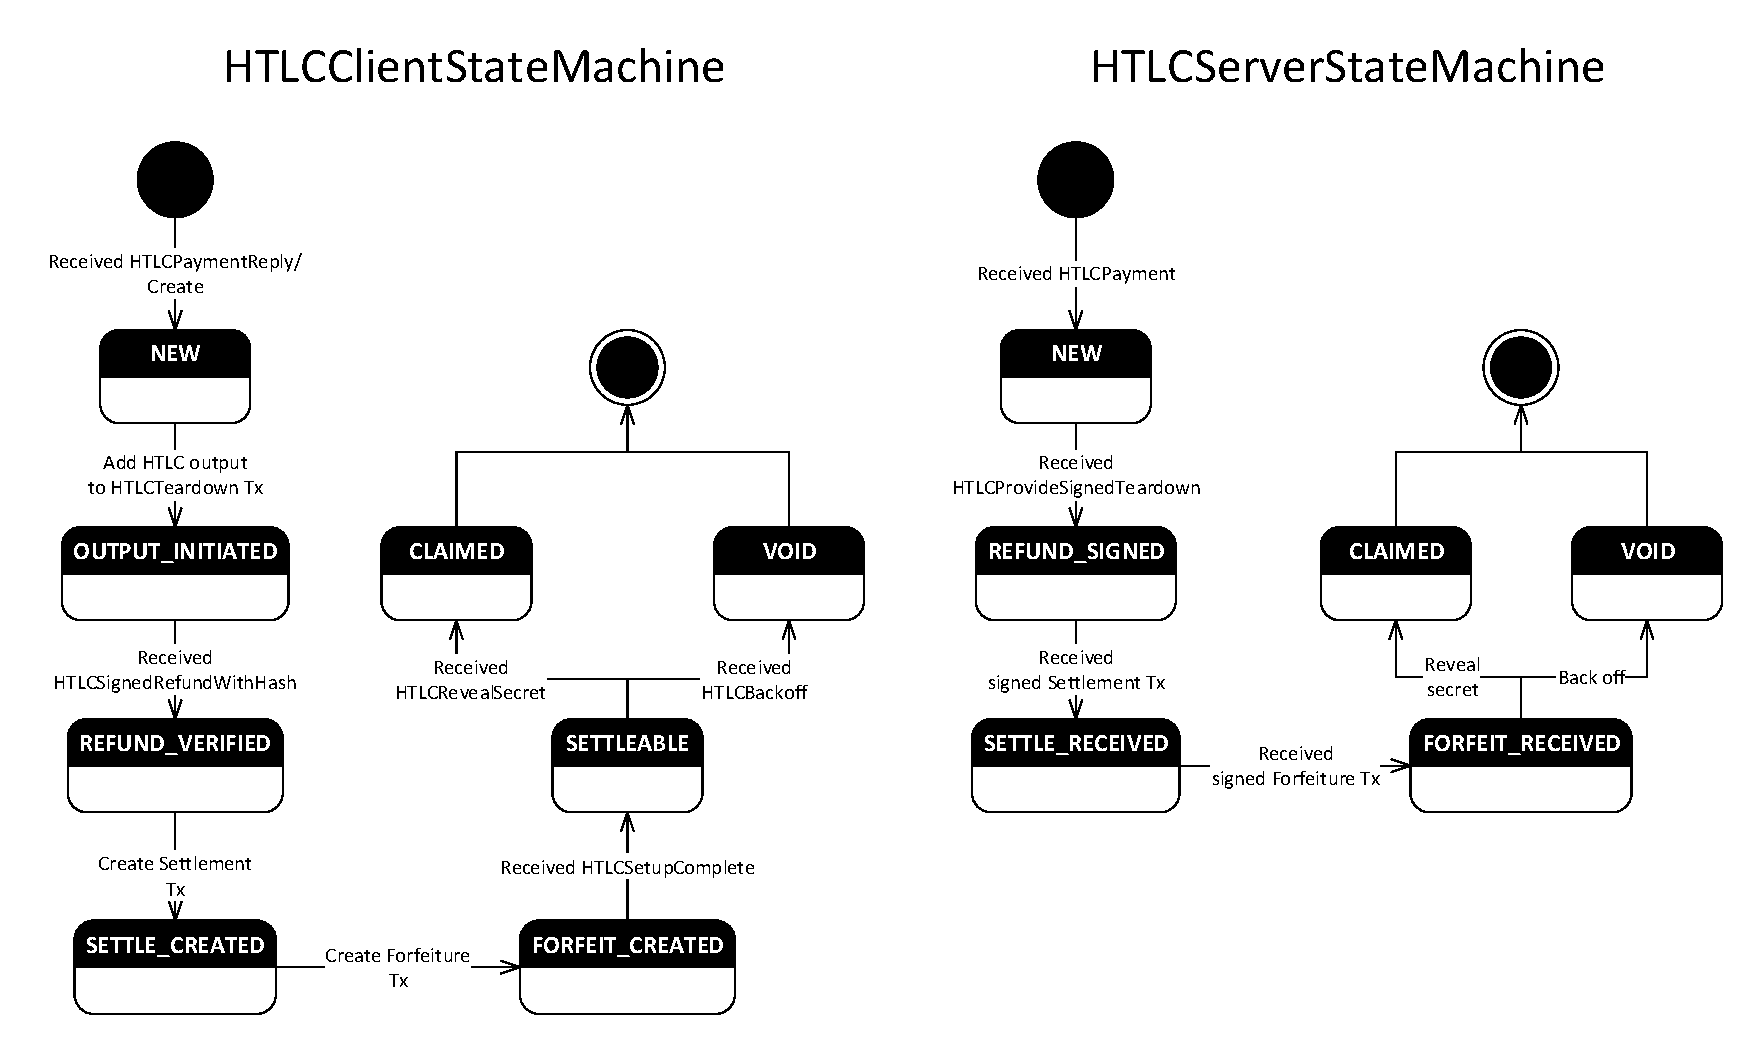
\includegraphics[width=\textwidth]{figures/HTLCStates}}
  \caption{HTLC State Machines for both client and server side}
  \label{fig:htlcstates}
\end{figure}

The client first sends an HTLCInit message containing a list of payments that were buffered during a 
previous active round. Each payment message contains a client request id, the value of the payment 
and information about the type of data that is requested in exchange. The server creates new 
HTLCServerStateMachine instances for each payment. Each HTLC is given an id, which is basically the 
hash of the secret. An HTLCInitReply message is then replied, mirroring back the client request id,
and sending the fresh HTLC id. From this stage on, each HTLC payment will be referenced by the server-generated id.

At this step, the client can also create HTLCClientStateMachine instances and update the HTLC setup transaction, adding
outputs for each initiated payment. The transaction is then signed and sent over to the server, together with the 
payment id and index of each active HTLC output.

Upon receiving the updated and signed HTLC setup transaction, the server can compute its hash,
and return signed HTLC refund transactions for all active HTLC payments (HTLCSignedRefundWithHash).
This step is necessary because removing outputs from the HTLC setup transaction invalidates the signatures 
of previously created HTLC refund, settlement and forfeiture transactions.

Once the client received the HTLCSignedRefundWithHash message, it stores the HTLC refund transactions and broadcasts them 
when their time lock expires if the HTLC setup transaction makes it to the block chain and the corresponding
HTLC outputs are not claimed by that time. The client can now recreate the HTLC forfeiture and settlement transactions
for all active HTLC payments, sign and hand them over to the server. After the server checks the signatures 
and stores the received transactions, it signals the client that the HTLC setup is complete.

\subsubsection{Claiming a payment}\label{claim}

\hspace*{12pt} After a successful setup, the server can initiate an update round to claim the payments 
from the HTLC outputs. To do so, it first sends an HTLCServerUpdate message to the client. 
It contains a list of HTLCSettlement and a list of HTLCForfeiture messages. 
Each reveal message indicates the id of the HTLC payment the server is claiming, together with the 
secret that hashes to its id. HTLCForfeiture messages contain the the ids of the HTLC payments that 
are voided and the fully signed HTLC forfeiture transactions, which guarantee the client that an older 
HTLC setup transaction will not be broadcast, should the secret be received at a later time.
They are sent by the server a fixed time before the channel expiration time and before the 
HTLC setup transaction is broadcast, such that the number of HTLC refund transactions that are 
later broadcast by the client is minimized. Thus, the HTLC refund transactions are kept off the block chain, 
and the server voluntarily opts to void the HTLC payments because it has not received the secret in time.

\begin{figure}[ht!]
  \centerline{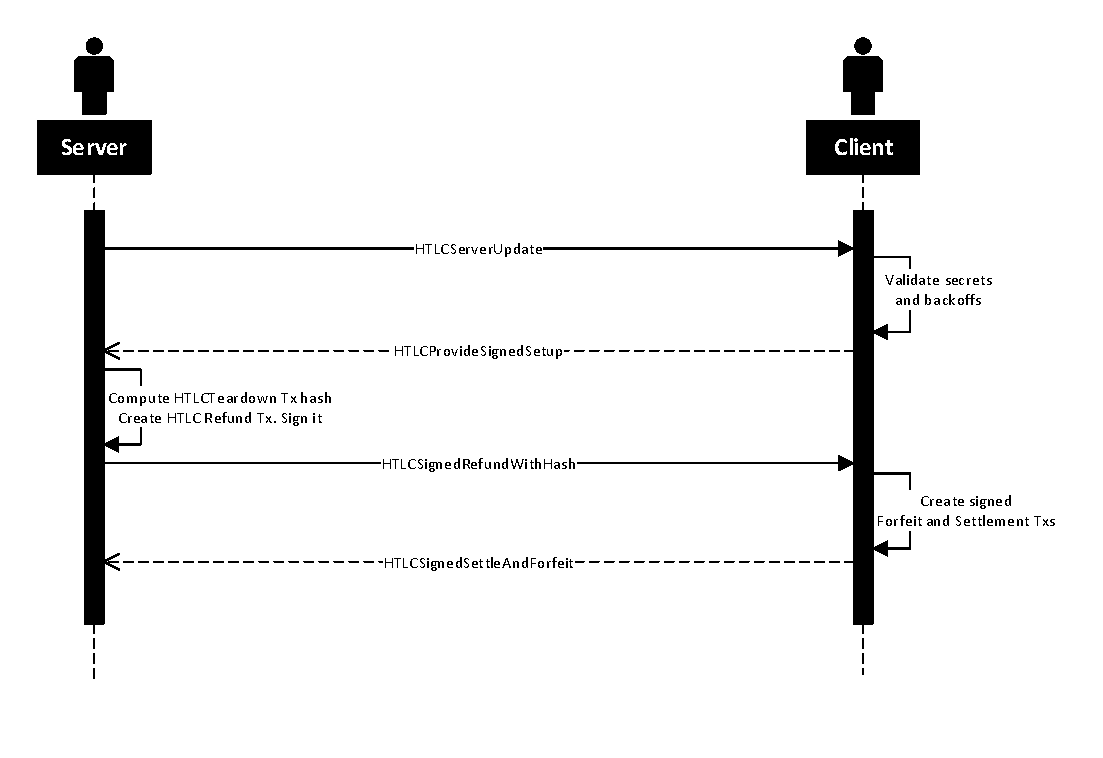
\includegraphics[width=\textwidth]{figures/HTLCClaimSeq}}
  \caption{HTLC Settlement and Forfeiture sequence diagram}
  \label{fig:htlcclaimseq}
\end{figure}

The client validates the received secrets and forfeiture transactions, and removes the HTLC outputs from the HTLC 
setup transaction accordingly. Forfeiture transactions are stored and hashes of older
HTLC setup transactions are followed on the block chain. Should any of them make it to the block chain,
the client will automatically broadcast the corresponding forfeiture transactions to get the funds back.
The updated HTLC setup transaction is then signed sent to the server using the HTLCProvideSignedSetup message. 
From here on, the process follows the same steps as in \ref{initpay}. 
The message succession is shown in Figure \ref{fig:htlcclaimseq}. 

\subsubsection{Closing the channel}

\hspace*{12pt} If the client wishes to close the payment channel before its expiration time, it can send
a close message to the server. Then the server can broadcast the most recent HTLC setup transaction to the
network, spending the bond transaction's output. If the server wishes to close the payment channel early, 
it simply broadcasts the most recent HTLC setup transaction and signals the client that the channel was closed
using the same close message. Should the HTLC setup transaction still contain HTLC outputs,
the server can claim them if it has the corresponding secrets using the HTLC settlement transactions, or,
if not, the client will get those funds back using the HTLC refund transactions.

\subsubsection{Data transmission}

\hspace*{12pt} In order to securely transmit the data that the client is issuing payments for, the client and the server need
a private, authentic out-of-band channel. In the HTLC payment setup phase, the data, encrypted with the HTLC secret,
would be transmitted to the client over the hub. Then, once the server has cleared the payment by revealing the secret,
the client can decrypt the previously received data. This ensures an atomic exchange of data for bitcoins.

\section {Application implementation}

\hspace*{12pt} Following the design introduced in the previous chapter and the client-server architecture described in the 
previous section, three different applications were developed, corresponding to each of the three components: 
buyer, central hub, and sensor node represented by an Android application on a device with a wide range 
of built-in sensors. In the next subsections, each application is presented in detail.

\subsection{Buyer application}

\hspace*{12pt} The buyer component was developed as a Java console application. From an architectural point of view,
it plays the role of a client in the payment protocol by connecting, initiating a micropayment channel with the hub and 
making payments to the hub in exchange for data.

\subsubsection{Running queries}
\hspace*{12pt} From the buyer driver console application, the following queries are available:
\begin{itemize}
 \item Node statistics. {\it STATS NODES} will display the number of connected sensor nodes with 
 list of sensor node ids. 
 \item Sensor statistics. {\it STATS SENSORS} will display the types of sensor data that are available for purchasing.
 \item Select queries. {\it SELECT SENSOR=\textless sensor\_type\textgreater } will display 
 all available nodes with the selected sensor type, together with id of the node it is available on, 
 and pricing information,
 \item Buy queries: {\it BUY \textless sensor\_type\textgreater FROM node\_id price} will 
 purchase the set of sensor data of the specified type from the node selected by id. 
 This query will return the asked data set.
\end{itemize}

\subsection{Hub application}

\hspace*{12pt} The hub application was developed as a Java application. It represents the discovery,
coordination and payment forwarding point of the developed system, with both a receiving (server) 
component from the perspective of the buyers, and a sending (client) component from the perspective 
of the sensor nodes.

To accommodate this design, the driver application, ChannelConnection, and PaymentChannel layers were modified.
A class diagram showing the modified layers can be found in the Appendix, Figure \ref{fig:hubuml}.
The ChannelStateMachine and HTLCStateMachines layers were integrated as originally designed.

At the application level, the hub establishes the connection to the Bitcoin network and synchronizes its local
block chain. In the ChannelConnection layer, two servers are run on two different ports for: one for connecting buyers,
and another one for sensor nodes. The layer also stores data such as mappings of sensor types to the devices that they 
are installed on, and pricing information, such that it can support node, sensor, and select queries. 
When a new buyer connects to the hub, a buyer-specific connection handler is used to establish a micropayment channel
and receive payments from the buyer. On the other hand, the sensor-specific handlers were adapted 
to act as servers connection-wise, but as clients in the payment protocol: they initiate 
micropayment channel establishment with the sensors and send payments to them.

A routing component keeps track of all payment ids and of the buyers and sensor nodes these payments 
are initiated between. This way, the destination of messages that need to be 
forwarded between the buyer and the Android components can be easily identified. If a message contains sub-messages
for multiple destinations, the router does deep-packet inspection, aggregates the sub-messages by destination, 
and finally forwards them.

\subsection{Android application}

\hspace*{12pt} The sensor node component was developed as an Android application, allowing the user of the app
to share sensor data in exchange for bitcoins. Since it represents the receiving party in the protocol,
it follows the server component design.

\begin{figure}[ht!]
  \centerline{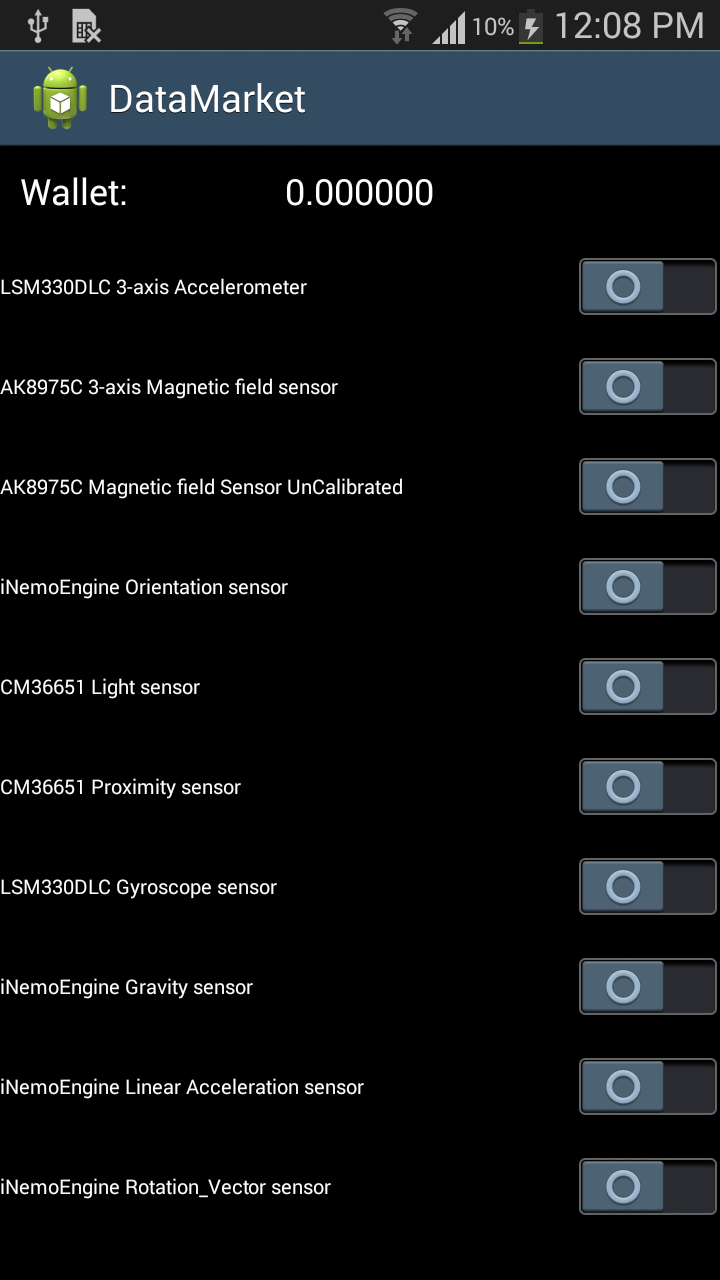
\includegraphics[width=.5\textwidth]{figures/app}}
  \caption{Android application user interface.}
  \label{fig:app}
\end{figure}

The user is given full choice regarding which data is shared to the interested buyers. The available device sensors
are detected at application start-up. The interface (Figure \ref{fig:app})
consists of a main view that allows the user to toggle between sharing or not sharing the data of each sensor.

The Bitcoin wallet is created on the first start and locally stored on the device. At this time, the user
can also set up prices for sensor sharing. Later on, the user can always go back and set new prices
using the settings option. At the top of the interface, the application displays 
the amount of bitcoins earned so far. 

The permissions needed by the developed Android application in order for the device to successfully participate
in the built system are specified in the Appendix \ref{permissions}.

\subsubsection{ChannelConnection layer adaptation}

\hspace*{12pt} In the original design, the ChannelConnection layer of the server is the one listening for new connections
from connecting clients. However, in this case, the Android application should be the one initiating the connection 
and registering to the central hub. In this regard, the ChannelConnection layer was adapted such that app is the one 
initializing the connection (connection client), but the payment protocol message exchange stays the same: 
the Android component is the receiving party, thus a payment server component.

\subsubsection{Connectivity}

\hspace*{12pt} To establish and maintain the TCP connection to the Hub, the code responsible for 
the Bitcoin operations was integrated into an Android remote service that starts at device boot-up. 
This ensures that the long-running operations do not block the application user interface and that 
the micropayment channel is kept alive even if the user closes the application.

When the service successfully establishes the TCP connection and sets up a micropayment channel with the hub,
the application is signaled. Then, the application registers the shared sensors to the hub. 
This is repeated every time the user changes its preferences in terms of the sensors data that is shared.

When the buyer requests some data from a specific sensor through the hub, the remote service can 
retrieve the data from the sensor listeners running in the application. 
Sensor listeners cache the data to allow instant data retrieval. A data container customizes the
number of data entries that are cached. The current implementation uses a EvictingQueue of a fixed size {\it K},
automatically maintaining the {\it K} most recent entries.

\subsection{Running the full-system protocol}

\begin{sidewaysfigure}[ht]
    \centerline{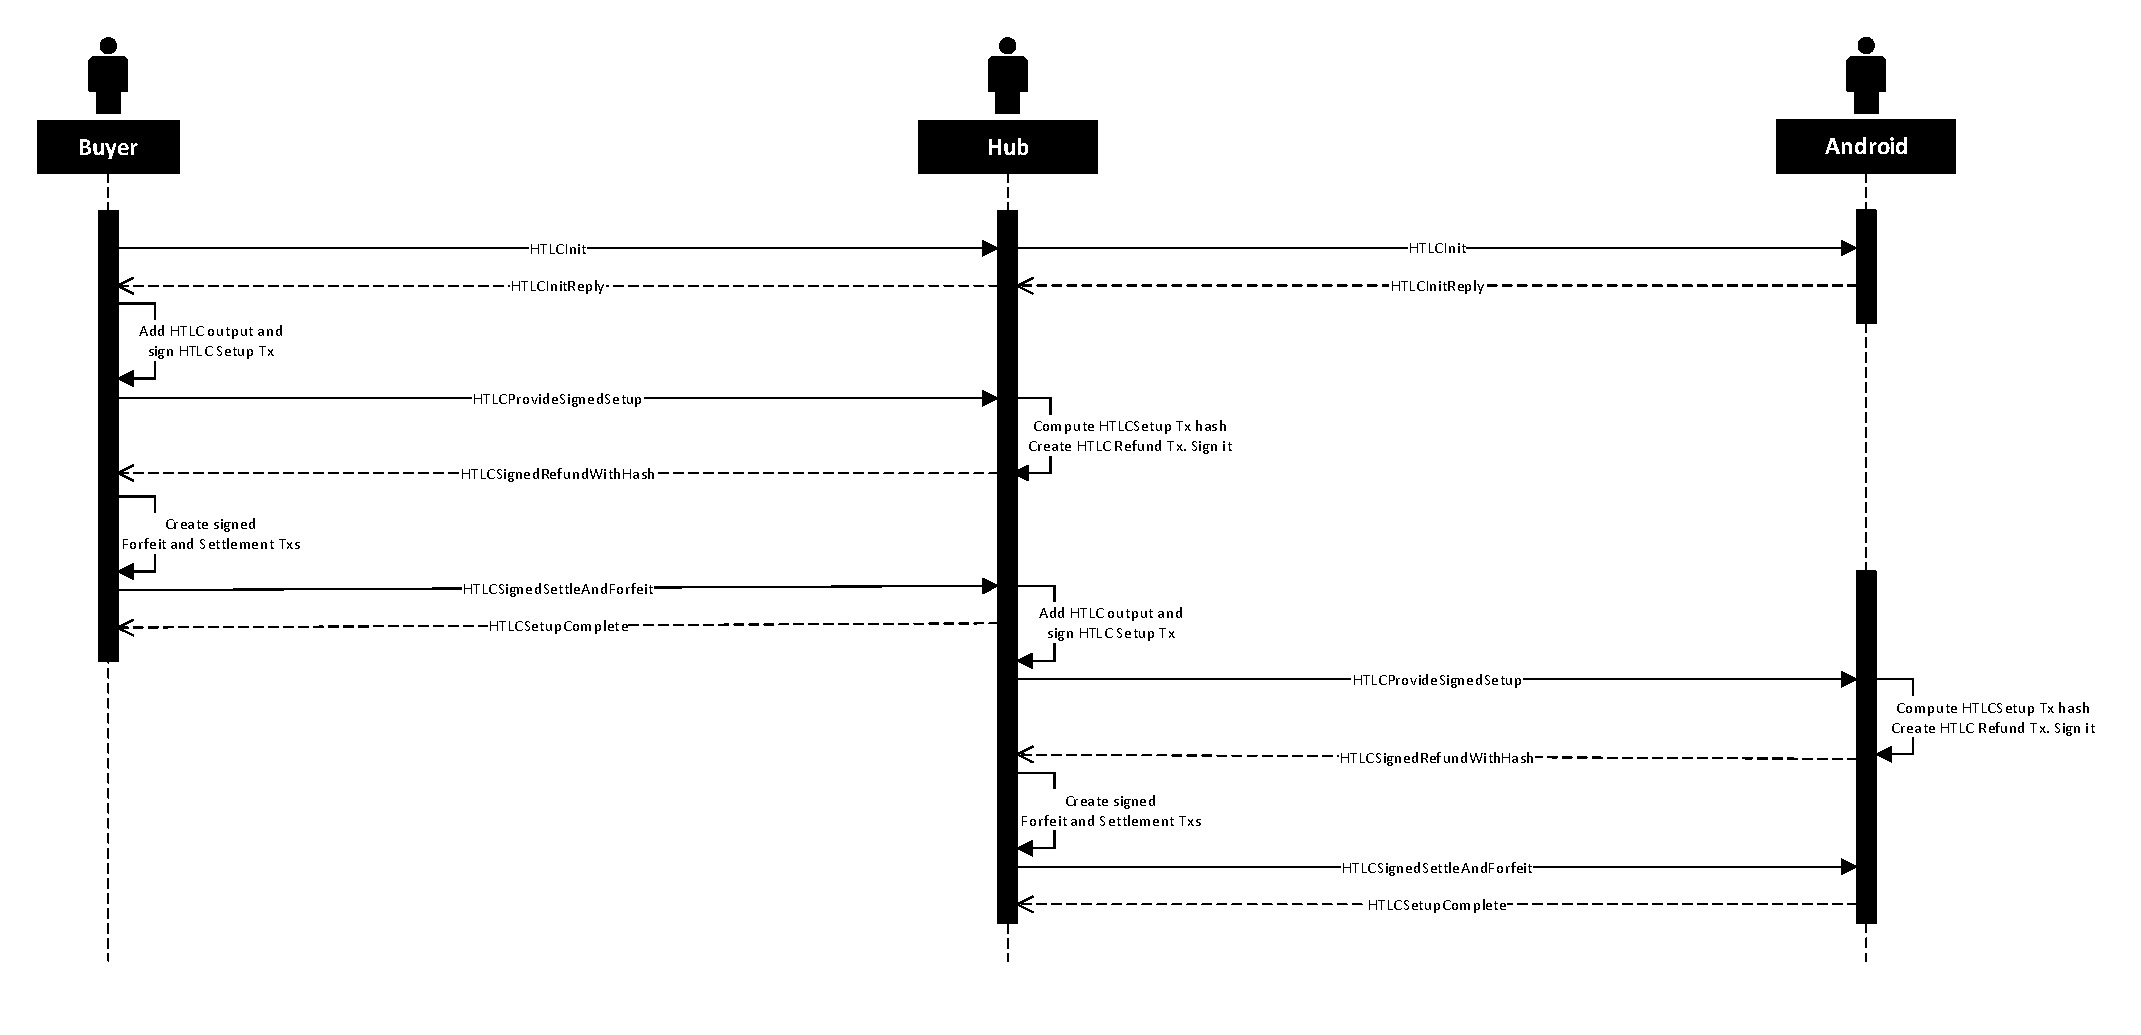
\includegraphics[width=\textwidth]{figures/FullHTLCSetup}}
    \caption{HTLC Full Setup sequence diagram}
  \label{fig:htlcfullsetup}
\end{sidewaysfigure}

\hspace*{12pt} In the full, three-component system, micropayment channels between the participants are 
established independently. Once at least one buyer and one Android device are connected and channels are in place, 
the buyer can initiate payments and receive the requested data in return. All requests are made during batched
update rounds.

Figure \ref{fig:htlcfullsetup} shows the message succession needed for the HTLC payment setup. The hub acts as a
transparent forwarding medium, passing through the messages between the buyer and the Android device and adjust
its state accordingly. First, the buyer sends an HTLCInit message. Upon receiving it, the hub forwards 
the HTLCInit to the Android device, which replies with an HTLCInitReply message. 
At this stage, the hub does not continue running the setup protocol with the Android device, 
but forwards back the reply, finally making it to the buyer. Now the buyer and the hub can run the 
HTLC payment setup protocol presented in detail in \ref{initpay}. 

After a successful setup, the hub can resume the paused setup protocol with the Android device. It is important
that the HTLC payment is first set up between the buyer and the hub to ensure the security of the protocol:
should the hub and the Android device first set up such a payment, nothing guarantees the hub
that it can claim the money from the buyer after it has paid the Android device.

When the Android device claims or voids some HTLC payments, it follows the exact pattern 
introduced in \ref{claim}. Only this time, after the hub receives and validates the HTLCServerUpdate message, 
it forwards it immediately to the buyer, and then continues with its update round. This way, the hub can run 
the update protocol simultaneously and the buyer can use the secret to decrypt the received data that was included in 
the HTLCInitReply message.

\chapter{Evaluation}

\hspace*{12pt} In this chapter, the system is evaluated both in terms of performance and security threats.

\section{Performance}

\hspace*{12pt} The performance of the built system was evaluated on the Bitcoin TestNet. 
The TestNet uses a different block chain with coins that have no value, making it an attractive platform 
for testing applications and experimenting with no financial loss.

\subsection{Setup}

For the performance evaluation, the following setup was used:
\begin{itemize}
  \item {\bf Central hub}. The hub was given 1000 bitcoins.
  \item {\bf Android component (Samsung GT-I9300)}. The component was connected to the central hub and registered with two sensors:
 {\it light} and {\it proximity}. It starts with an empty wallet.
  \item {\bf Buyers}. 100 buyers were connected to the hub. Each was given 1 bitcoin.
\end{itemize}

The central hub and the buyer application were run on the same local machine. All three components were 
connected to the same local Internet network.

\subsubsection{Micropayment channels}

\hspace*{12pt} The time needed to set up and close the micropayment channels between the buyers and the hub was measured. 
In the {\it bitcoinj} library, the server signals the client that the micropayment channel has been opened 
immediately after the multi-signature contract propagated to the network. 
However, in order to be truly secure, the channel should only be considered open after the transaction
was included in a block in the block chain. Measurements were made according to this observation.

\subsubsection{Making queries}

\hspace*{12pt} Each buyer was set up such that it chooses one of the four available queries with equal probability
every 5 seconds, putting a constant load on the system:
\begin{itemize}
 \item {\it STATS NODES}.
 \item {\it STATS SENSORS}.
 \item {\it SELECT SENSOR=\textless sensor\_type\textgreater}. Where \textless sensor\_type\textgreater 
 is randomly chosen between the two available sensors.
 \item {\it BUY \textless sensor\_type\textgreater \ FROM node\_id price}. The price was fixed to {\it 1} microbitcoin.
\end{itemize}

The following data was collected during the experiment:
\begin{itemize}
 \item {\it Response times} for each query type.
 \item {\it HTLC setup times}. The time needed to set up the HTLCs was measured both between each pair of components, 
 and on the complete path.
 \item {\it HTLC resolution times}. The time needed to teardown the HTLCs and restore the HTLC setup transaction 
 to a secure state was measured.
\end{itemize}

\subsection{Results}

\subsubsection{Micropayment channels}

\hspace*{12pt} As it can be seen in Table \ref{microsetup}, the time spent by buyers to establish 
a micropayment channel with the central hub and close it at the end of a session varies 
from a couple of minutes for up to ten minutes. This variation is given by the probabilistic nature 
of proof of work performed by the miners to include transactions in new blocks. In addition,
the TestNet tends to be rather unstable due to experimental work. In the main Bitcoin network, the expected time
to get a transaction included in the block chain is 10 minutes.

\begin{table}[!ht]
\centering
\begin{tabular}{|l|r|r|}
\hline
{\bf Micropayment channel}   	& \multicolumn{1}{l|}{{\bf Setup}} & \multicolumn{1}{l|}{{\bf Close}} \\ \hline
Mean            		& 107.11 s	    	           &   977.83 s          \\ \hline
St. Dev.        		& 5.16 s	                   &   3.34 s         \\ \hline
\end{tabular}
\caption{Micropayment channel setup and close time average and standard deviation on TestNet.}
\label{microsetup}
\end{table}

\subsubsection{Queries} 

\hspace*{12pt} Table \ref{simplequeries} shows the obtained response times for each query type.
To get a better understanding of where is most of the response time for buy queries is 
spent in the system, a breakdown of the measurements is given for each hop on the payment path in Table \ref{breakdown}.

\begin{table}[H]
\centering
\begin{tabular}{|l|c|r|r|}
\hline
{\bf Query type}   & {\bf Nr. of queries} & \multicolumn{1}{l|}{{\bf Mean}} & \multicolumn{1}{l|}{{\bf St. Dev.}} \\ \hline
Select		   & 853                  & 41.6 ms                  & 2.9 ms                      \\ \hline
Node stats         & 863                  & 40.9 ms                  & 2.7 ms                      \\ \hline
Sensor stats       & 922                  & 40.8 ms                  & 4.3 ms                      \\ \hline
Buy  		   & 744 		  & 1497.9 ms		    & 229.9 ms			  \\ \hline
\end{tabular}
\caption{Mean and standard deviation of the response times for select, node and sensor, and buy queries.}
\label{simplequeries}
\end{table}

\begin{table}[H]
\centering
\begin{tabular}{|l|r|r|}
\hline
{\bf Buy queries breakdown} & \multicolumn{1}{l|}{{\bf Mean}} & \multicolumn{1}{l|}{{\bf St. Dev.}} \\ \hline
Full setup                  & 1054.6 ms                & 151.4 ms                     \\ \hline
Buyer-Hub setup             & 479.3 ms                 & 78.8 ms                      \\ \hline
Hub-Sensor setup            & 1015.1 ms                & 151.4 ms                     \\ \hline
Hub-Sensor teardown         & 199.6 ms                 & 68.3 ms                      \\ \hline
Buyer-Hub teardown          & 146.6 ms                 & 10.1 ms                      \\ \hline
\end{tabular}
\caption{Buy query response time breakdown by payment hop.}
\label{breakdown}
\end{table}

\subsubsection{Full communication trace}

\hspace*{12pt} In this section, a full communication trace is inferred from the obtained mean results. A buyer session
is expected to have the following pattern:
\begin{itemize}
 \item {\it Establish a micropayment channel} with the hub. This step takes place on the block chain because it needs
 the bond transaction to be confirmed by the network to lock in the buyer's funds.
 \item {\it Run several buy queries}. This step runs completely off the block chain.
 \item {\it Close the micropayment channel}. The settlement of the channel involves broadcasting the latest
 version of the HTLC setup transaction, taking place on the block chain.
\end{itemize}

\begin{figure}[h]
  \centerline{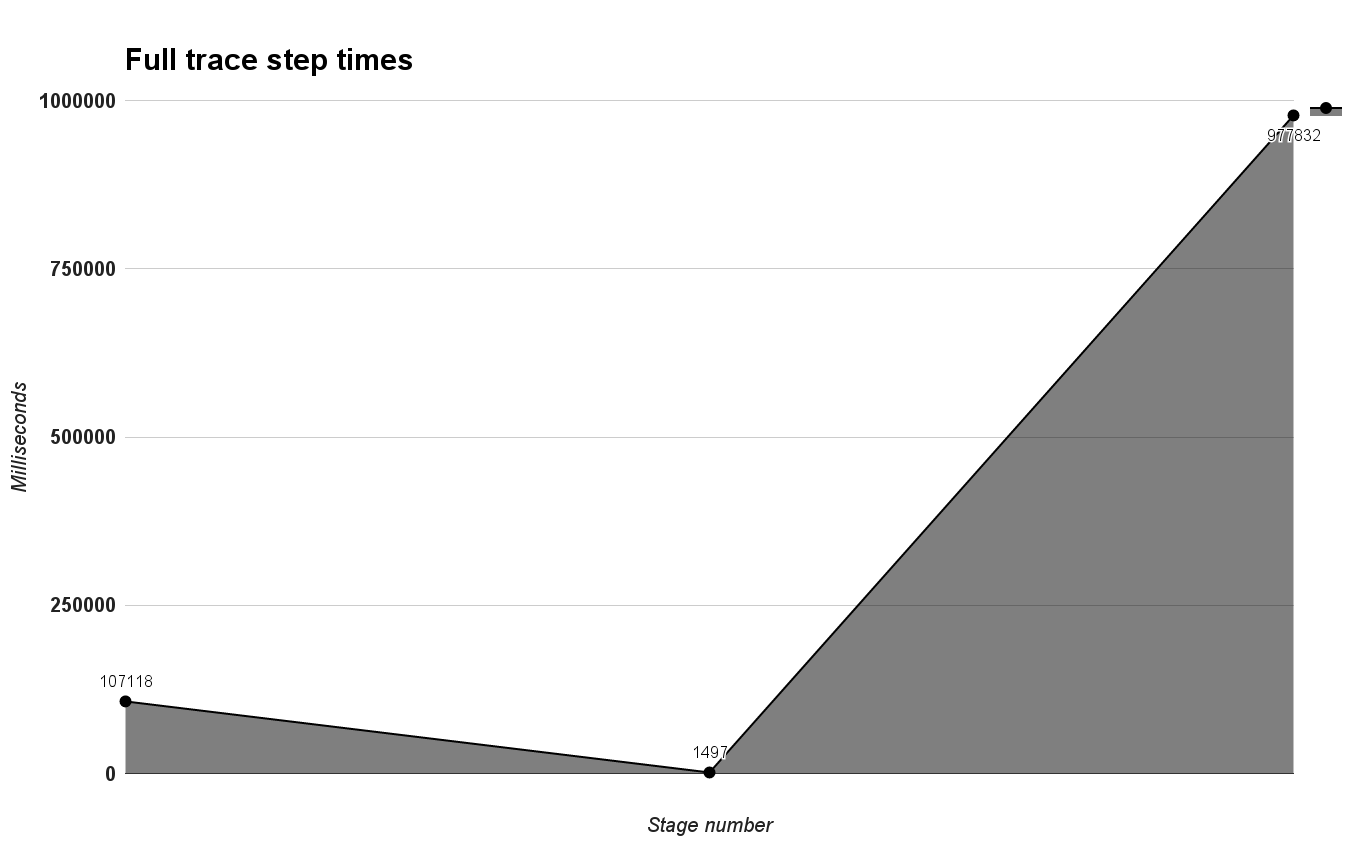
\includegraphics[width=\textwidth]{figures/trace}}
  \caption{Full communication trace using mean measurement values.}
  \label{fig:trace}
\end{figure}

Figure \ref{fig:trace} shows the average times for a full communication trace based on the described pattern. For each pattern
step, the mean values obtained from the previous evaluation results are used.

\subsubsection{Discussion}

\hspace*{12pt} An important observation regarding the performance results is the unpredictable and high transaction 
confirmation times on the Bitcoin TestNet network.
If each payment in the system was included in an individual transaction, the overall experience of the buyer would 
be poor, encountering high fees and query times, and possibly getting transactions rejected by the system because 
of the anti-flood algorithms running on the network.

On the other hand, micropayment channels only require one transaction to be confirmed, locking in the funds 
allocated by the buyer. After this setup time, queries and payments can be made securely and very fast, 
without broadcasting any transaction to the block chain. This can be observed by analyzing Figure \ref{fig:trace}:
after the setup time, buy queries are executed very fast. When the channel needs to be closed, the broadcast
of the final transaction takes again a long time to be included in the block chain. If the expected transaction
confirmation time of 10 minutes from the main Bitcoin network is considered, the payments done through the built system
are approximately $400$ times faster.

By further analyzing the obtained performance results, it can be observed that most of the time in a buy query is spent
during the HTLC setup phase, which includes initiating a payment, updating the HTLC setup transaction and the
exchange of HTLC refund, settlement, and forfeiture transactions on the full path. 
In fact, the setup phase represents $67\%$ out of the total buy query time. 
This is mainly due to the fact that the sensor node has to wait until the HTLC is successfully set 
up between the buyer and the hub, before it can resume the HTLC setup process with the hub. 
Without this condition, the node cannot be assured that it can claim the created HTLC output from the hub.

In the HTLC teardown phase, the hub and sensor node took an average of $199.6$ ms, 
and the buyers and the hub $146.6$ ms to get back to a secure state in the channel. These times
are dominated by the cryptographic operations during transaction signing. The performance
of the two hops is more similar because this stage is parallelized: after the hub receives the secret 
from the sensor node, it validates it and immediately forwards it to the buyer instead of waiting to 
clear the HTLC output from the HTLC setup transaction. When the buyer also received the secret, 
it can independently update its state with the hub. On average, the teardown stage between the hub and 
the sensor node takes longer because the latter has a poorer hardware performance.

\section{Protocol vulnerabilities}

\hspace*{12pt} In this section, the vulnerabilities of the built system are briefly evaluated and countermeasures
for each such vulnerability are introduced.

\subsection{Payment security}

\hspace*{12pt} Because of the Bitcoin malleability issue, the payment setup stage of the protocol has a major caveat: 
it sends over the signed HTLC setup transaction before having any signed HTLC refund transaction that 
protects the client in case the server decides to lock away the funds in the HTLC outputs indefinitely. 
It cannot be avoided without the malleability fix, because the client cannot create by itself an 
HTLC refund transaction that spends from the HTLC output: the HTLC setup transaction spends from the 
multisig output between the two parties, and it needs to be fully signed for the refund transaction to correctly 
reference it by its hash. Thus, in the current implementation, a minimal amount of trust is needed in 
the server component, that it will indeed sign, compute the hash of the HTLC setup transaction,
and return signed HTLC refund transactions for all active HTLC payments. The amount of trust in the server,
however, can be adjusted by limiting the number of active HTLC payments at a time.
Once the client received the HTLC setup transaction hash and HTLC refund transactions for each payment, 
the protocol is back to a secure state.

\subsection{Flow messages}

\hspace*{12pt} In the current proof-of-concept, the system transmits all messages unauthenticated and 
unencrypted. An attacker could eavesdrop, modify, or inject messages on the used TCP connections, 
gathering information and learning about what is happening in the system. Even though the messages are 
serialized in binary format, the format is publicly-known and can be easily decoded. A countermeasure 
for this vulnerability is to use socket layer encryption.

\subsection{Sensor data}

\subsubsection{Data validity}

\hspace*{12pt} The introduced protocol guarantees the buyer that it will get the data it paid for. In the payment setup phase,
the data encrypted with the secret is transmitted to the buyer. If the data is not received during this stage, the buyer
can simply choose not to continue running the rest of the payment protocol and use the channel refund transaction to get its
money back.

Assuming that the payment is successful, the buyer will receive the secret to decrypt the data it is in possession of.
However, the atomic exchange of data for bitcoins does not guarantee the validity of that piece of data. The data could be 
corrupt, random bytes containing no real sensor data, or could be simply faked by nodes with no sensors.

In order to mitigate this, it is important to consider a reputation system on the central hub. Since each sensor is registered
upon connecting with a unique device id that the buyers can use to get specific sensor data from, 
the hub could also publish reputation scores for each sensor node on the {\it select} queries. Then, after consulting the 
scores, the buyer can make an educated choice regarding the nodes it buys data from.

\subsubsection{Data confidentiality}

\hspace*{12pt} In the built proof-of-concept, the data is transmitted between the sensor nodes and the buyers through the
central hub. Since the secret disclosure is done backwards on the full payment path, the hub will also come into possession
of the secret and can decrypt the data purchased by the buyer. This violates the confidentiality since the data is
disclosed to an unauthorized entity. 

A possible countermeasure for this issue is to nest symmetric key encryption and public key encryption. 
The secret generating the hash commit is used as the key in the symmetric key encryption, whereas the resulting
cypher-text is encrypted again using the public key of the buyer. When initializing a new payment,
the buyer would transmit its public key to the hub, which then forwards it to the sensor node. At this stage,
the node can encrypt the data with the generated secret, and then encrypt it again using the received public key of the buyer.
This way, even if the hub attempts to decrypt the upper layer of the data, it cannot fully decrypt it since it does not have
the corresponding private key.

Another option is to combine the public key of the buyer with the payment secret. This can be done because the public
key cryptography based on elliptic curve is an additive homomorphism and allows adding the secret to the private
and public keys separately. Using the combined key, the sensor node can encrypt the data and send it to the buyer 
through the hub. Since only the buyer is in possession of the corresponding private key, it is the only one able 
to decrypt the received data.

\chapter{Conclusion}

\hspace*{12pt} The Internet of Things is expected to consist of networks encompassing billions of sensor nodes generating
huge amounts of data. Following the Sensing as a Service concept, the sensor nodes can engender global data markets
by offering their data as a service to interested entities for an agreed cost.

In this thesis, a centralized, low-trust and secure scheme has been built to incentivize sensor 
nodes to share sensed data in exchange for bitcoins. The scheme combines two existing Bitcoin constructs:
micropayment channels and hashed timelock contracts. Scalability is achieved by avoiding 
the broadcast of each micro-transaction through the use of the micropayment channel construct. 
The funds transferred between sensor nodes and interested buyers are transparently forwarded through a 
central hub that also acts as a coordinator and discovery point. End-to-end security of the payments is 
ensured by the use of hashed timelock contracts, broadcasting intermediary transactions only to 
handle conflict resolution. In order to be truly secure, the protocol needs a fix for the malleability issue of Bitcoin.
Otherwise, the receiver part can lock away payments indefinitely. Without the fix, however, this threat is minimized 
by adjusting the number of payments that can be active at a time.

A proof-of-concept of the proposed scheme has been implemented, using one component acting as a buyer, another one as
the central coordinator, and an Android device running a specialized application as a sensor node. By querying
the hub, the buyer can obtain information about available sensor data and purchase the data it is interested in.
An analysis of the response time of the built system has yielded that fund transfers between the buyers and 
the data providers in the system achieve real-time performance. 

The developed protocol meets the individual needs of repeated small value transactions in the Internet of Things scenario
and can be executed on small devices such as smartphones. By focusing future research on improving performance
and minimizing power consumption on the sensor system components, the protocol can be tailored for small sensor
nodes capable of cryptographic operations and can be adopted ubiquitously, opening up new opportunities 
in data sharing and enabling access to sensor data at an unprecedented scale. 

% This displays the bibliography for all cited external documents. 
%All references have to be defined in the file references.bib and can then be cited from within this document.
\bibliographystyle{plainurl}
\bibliography{references}

% This creates an appendix chapter, comment if not needed.
\appendix
\chapter{Appendix Chapter}

\section{HTLC Transactions}

\begin{figure}[h]
  \centerline{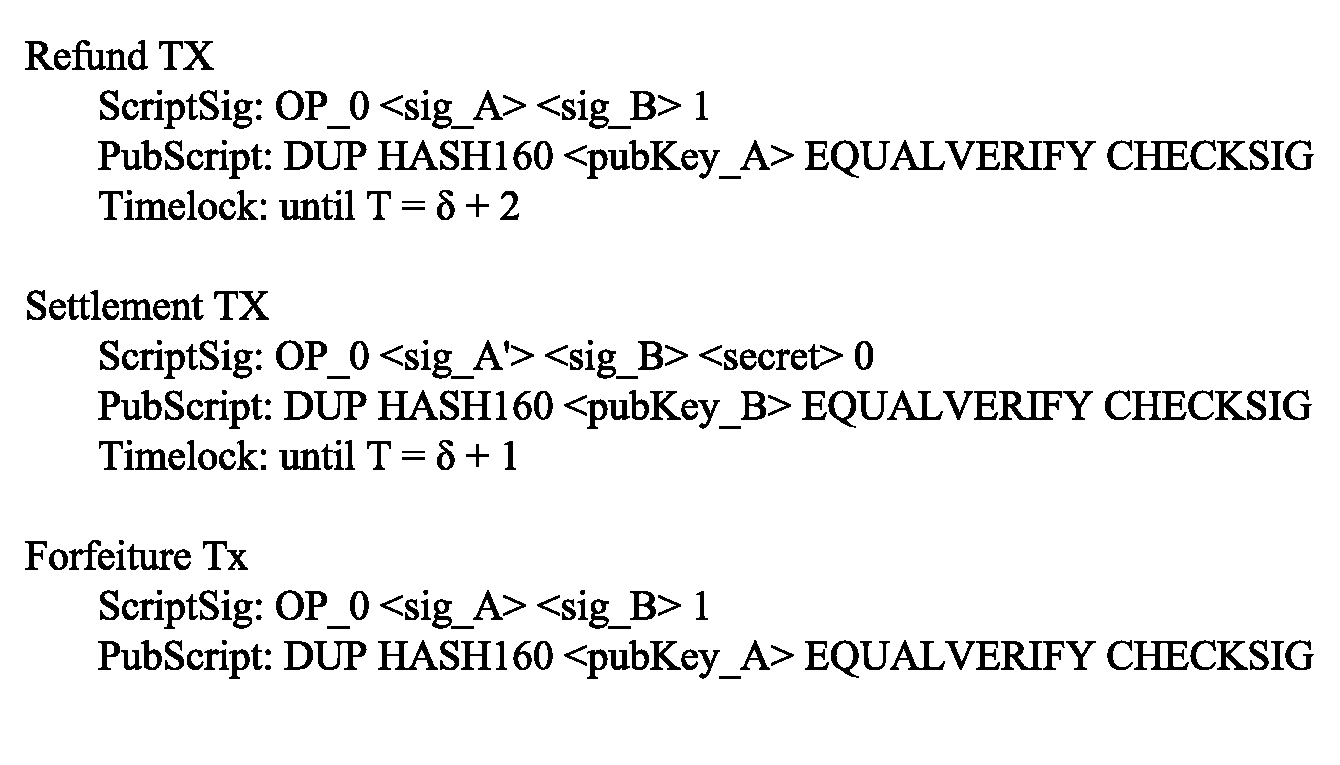
\includegraphics[width=\textwidth]{figures/HTLCPubScripts}}
  \caption{The HTLC refund, settlement and forfeiture transactions.}
  \label{fig:pubscripts}
\end{figure}

\section{Protobuf messages}\label{protobuf}

\hspace*{12pt} All messages prefixed with {\it HTLC*} are introduced for the scope of this work, while the others
already existed in the current version of the library.

\lstinputlisting{protobuf.txt}

\section{Android application}

\subsection{Permission requirements} \label{permissions}
\begin{itemize}
 \item {\bf android.permission.INTERNET}. The application needs Internet connectivity at all times.
 \item {\bf android.permission.WRITE\_EXTERNAL\_STORAGE}. The application needs permission to store and update the wallet
 and block chain files.
 \item {\bf android.permission.RECEIVE\_BOOT\_COMPLETED}. The application needs to receive the BOOT\_COMPLETED signal
 to initialize the micropayment channel to the hub.
\end{itemize}

\section{UML diagrams}

\begin{figure}[h]
  \centerline{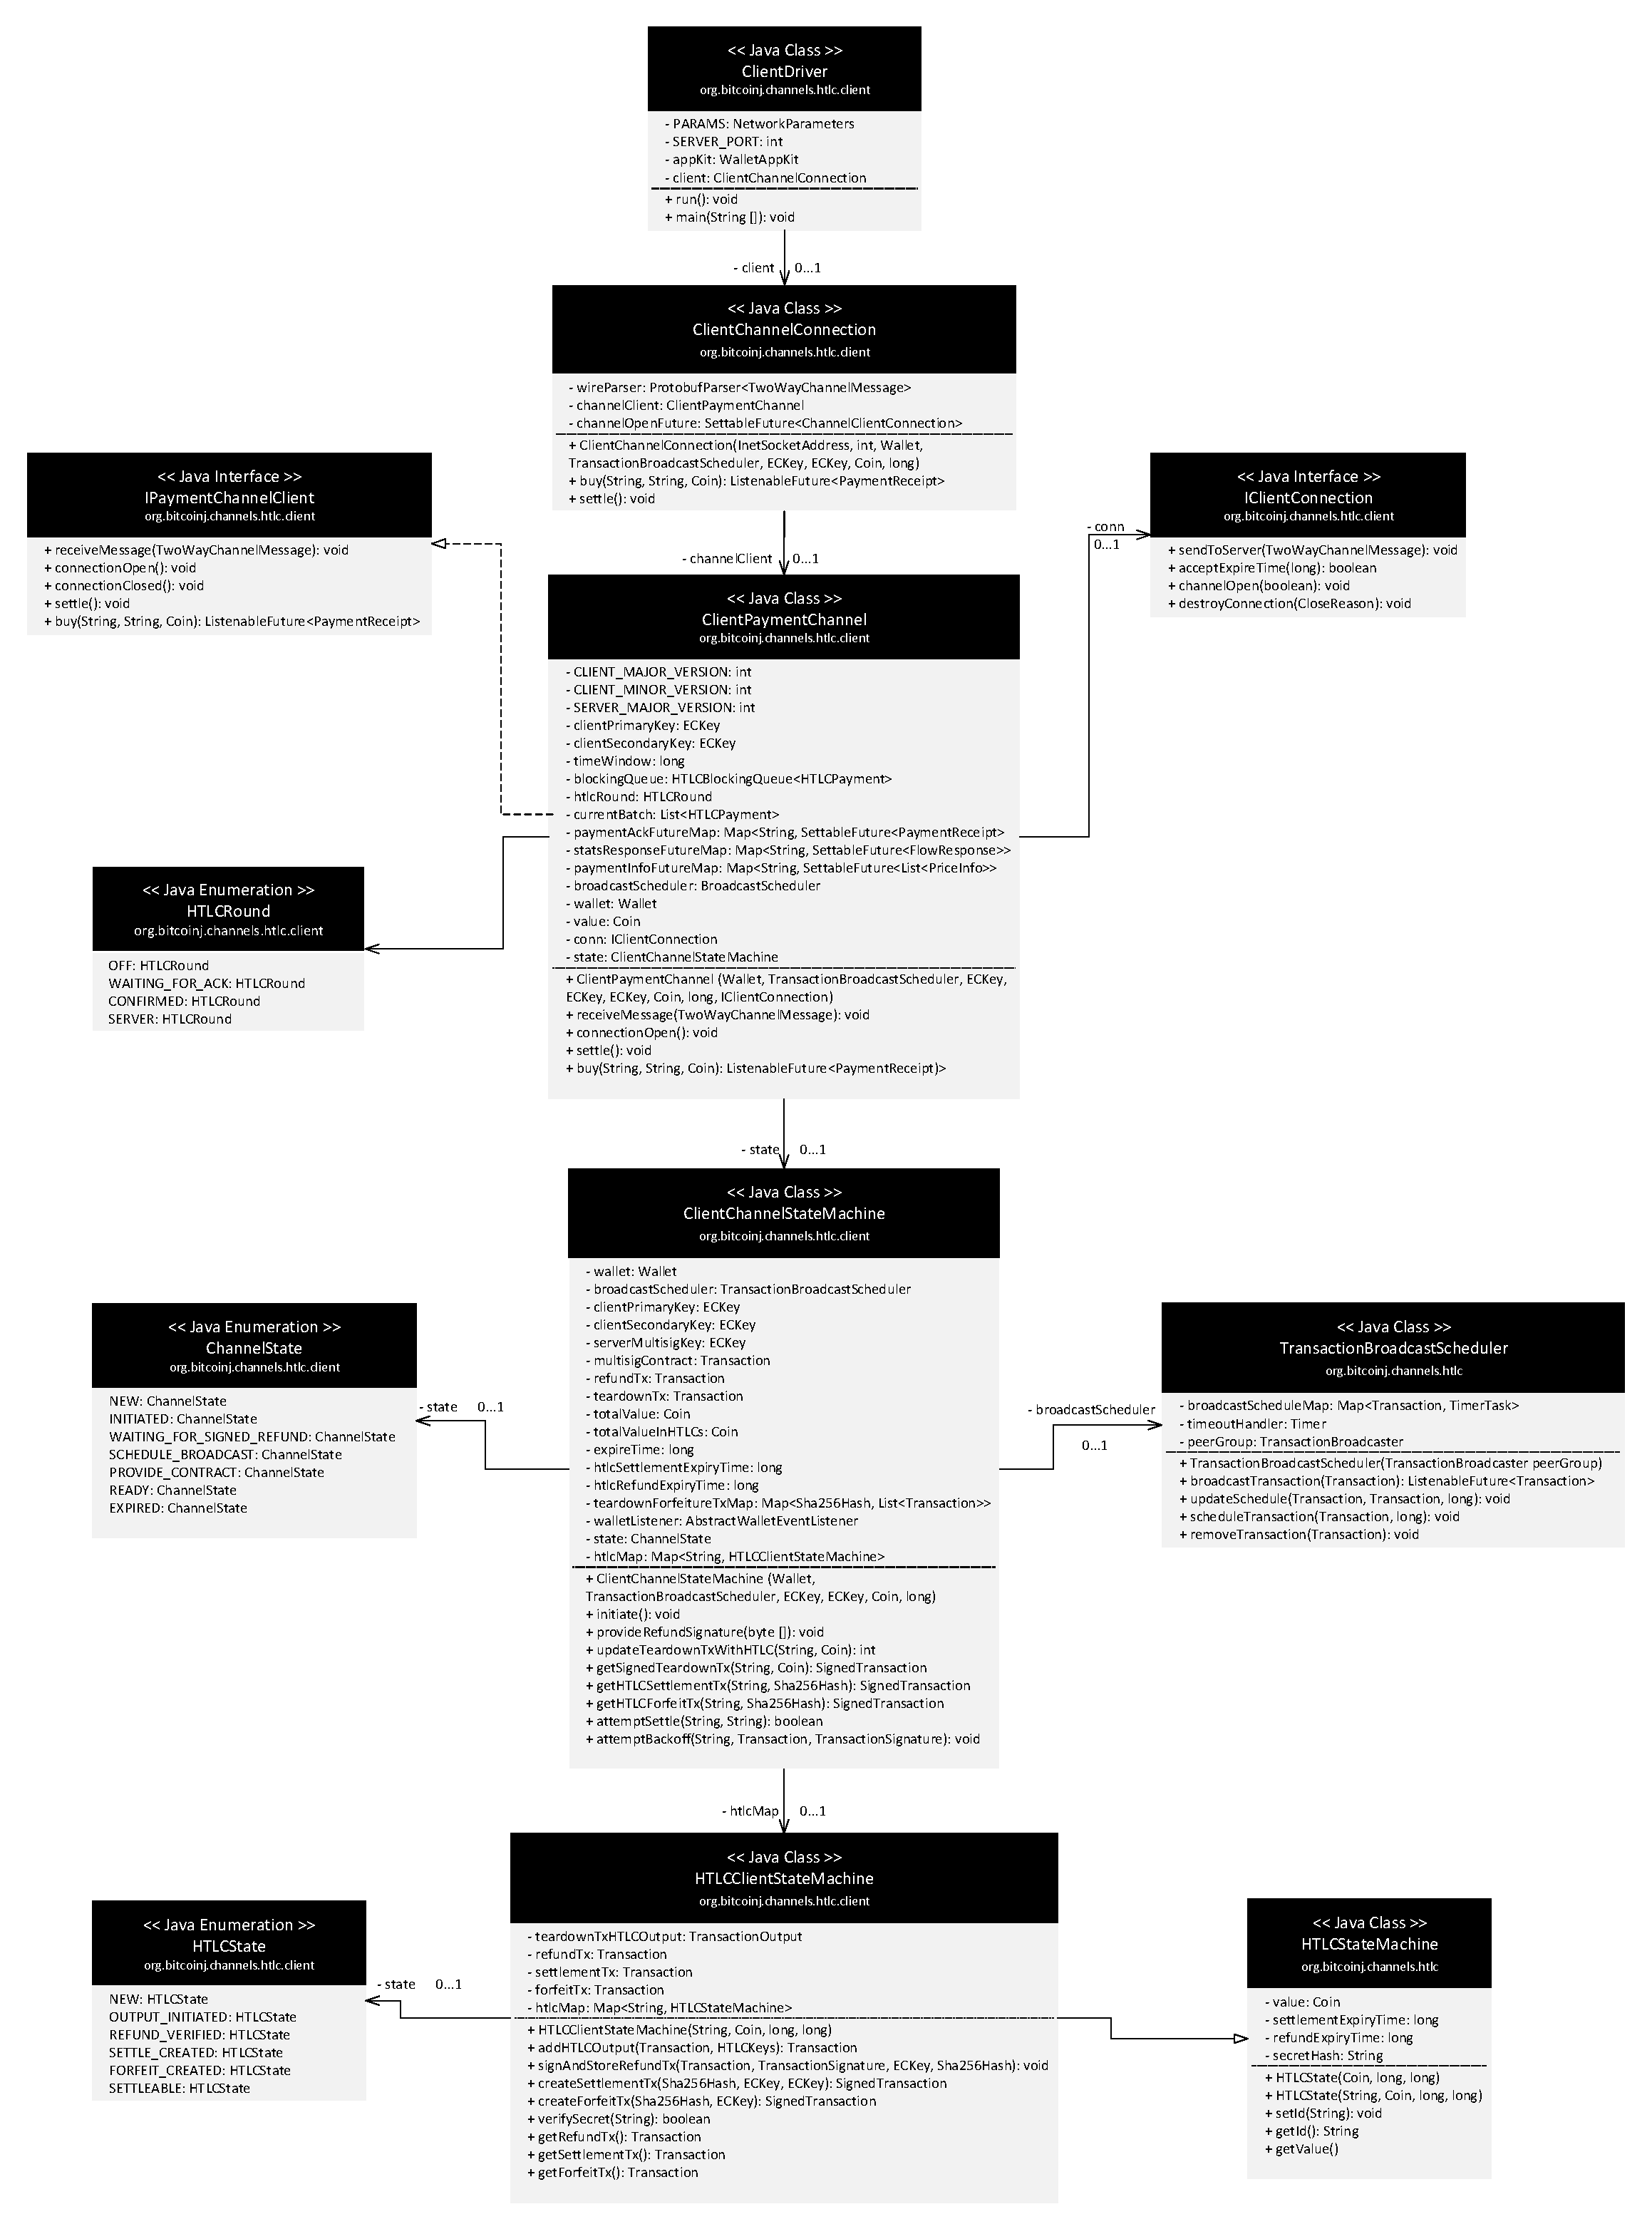
\includegraphics[width=1.2\textwidth]{figures/ClientUML}}
  \caption{UML class diagram of the Client component}
  \label{fig:clientuml}
\end{figure}

\begin{figure}[h]
  \centerline{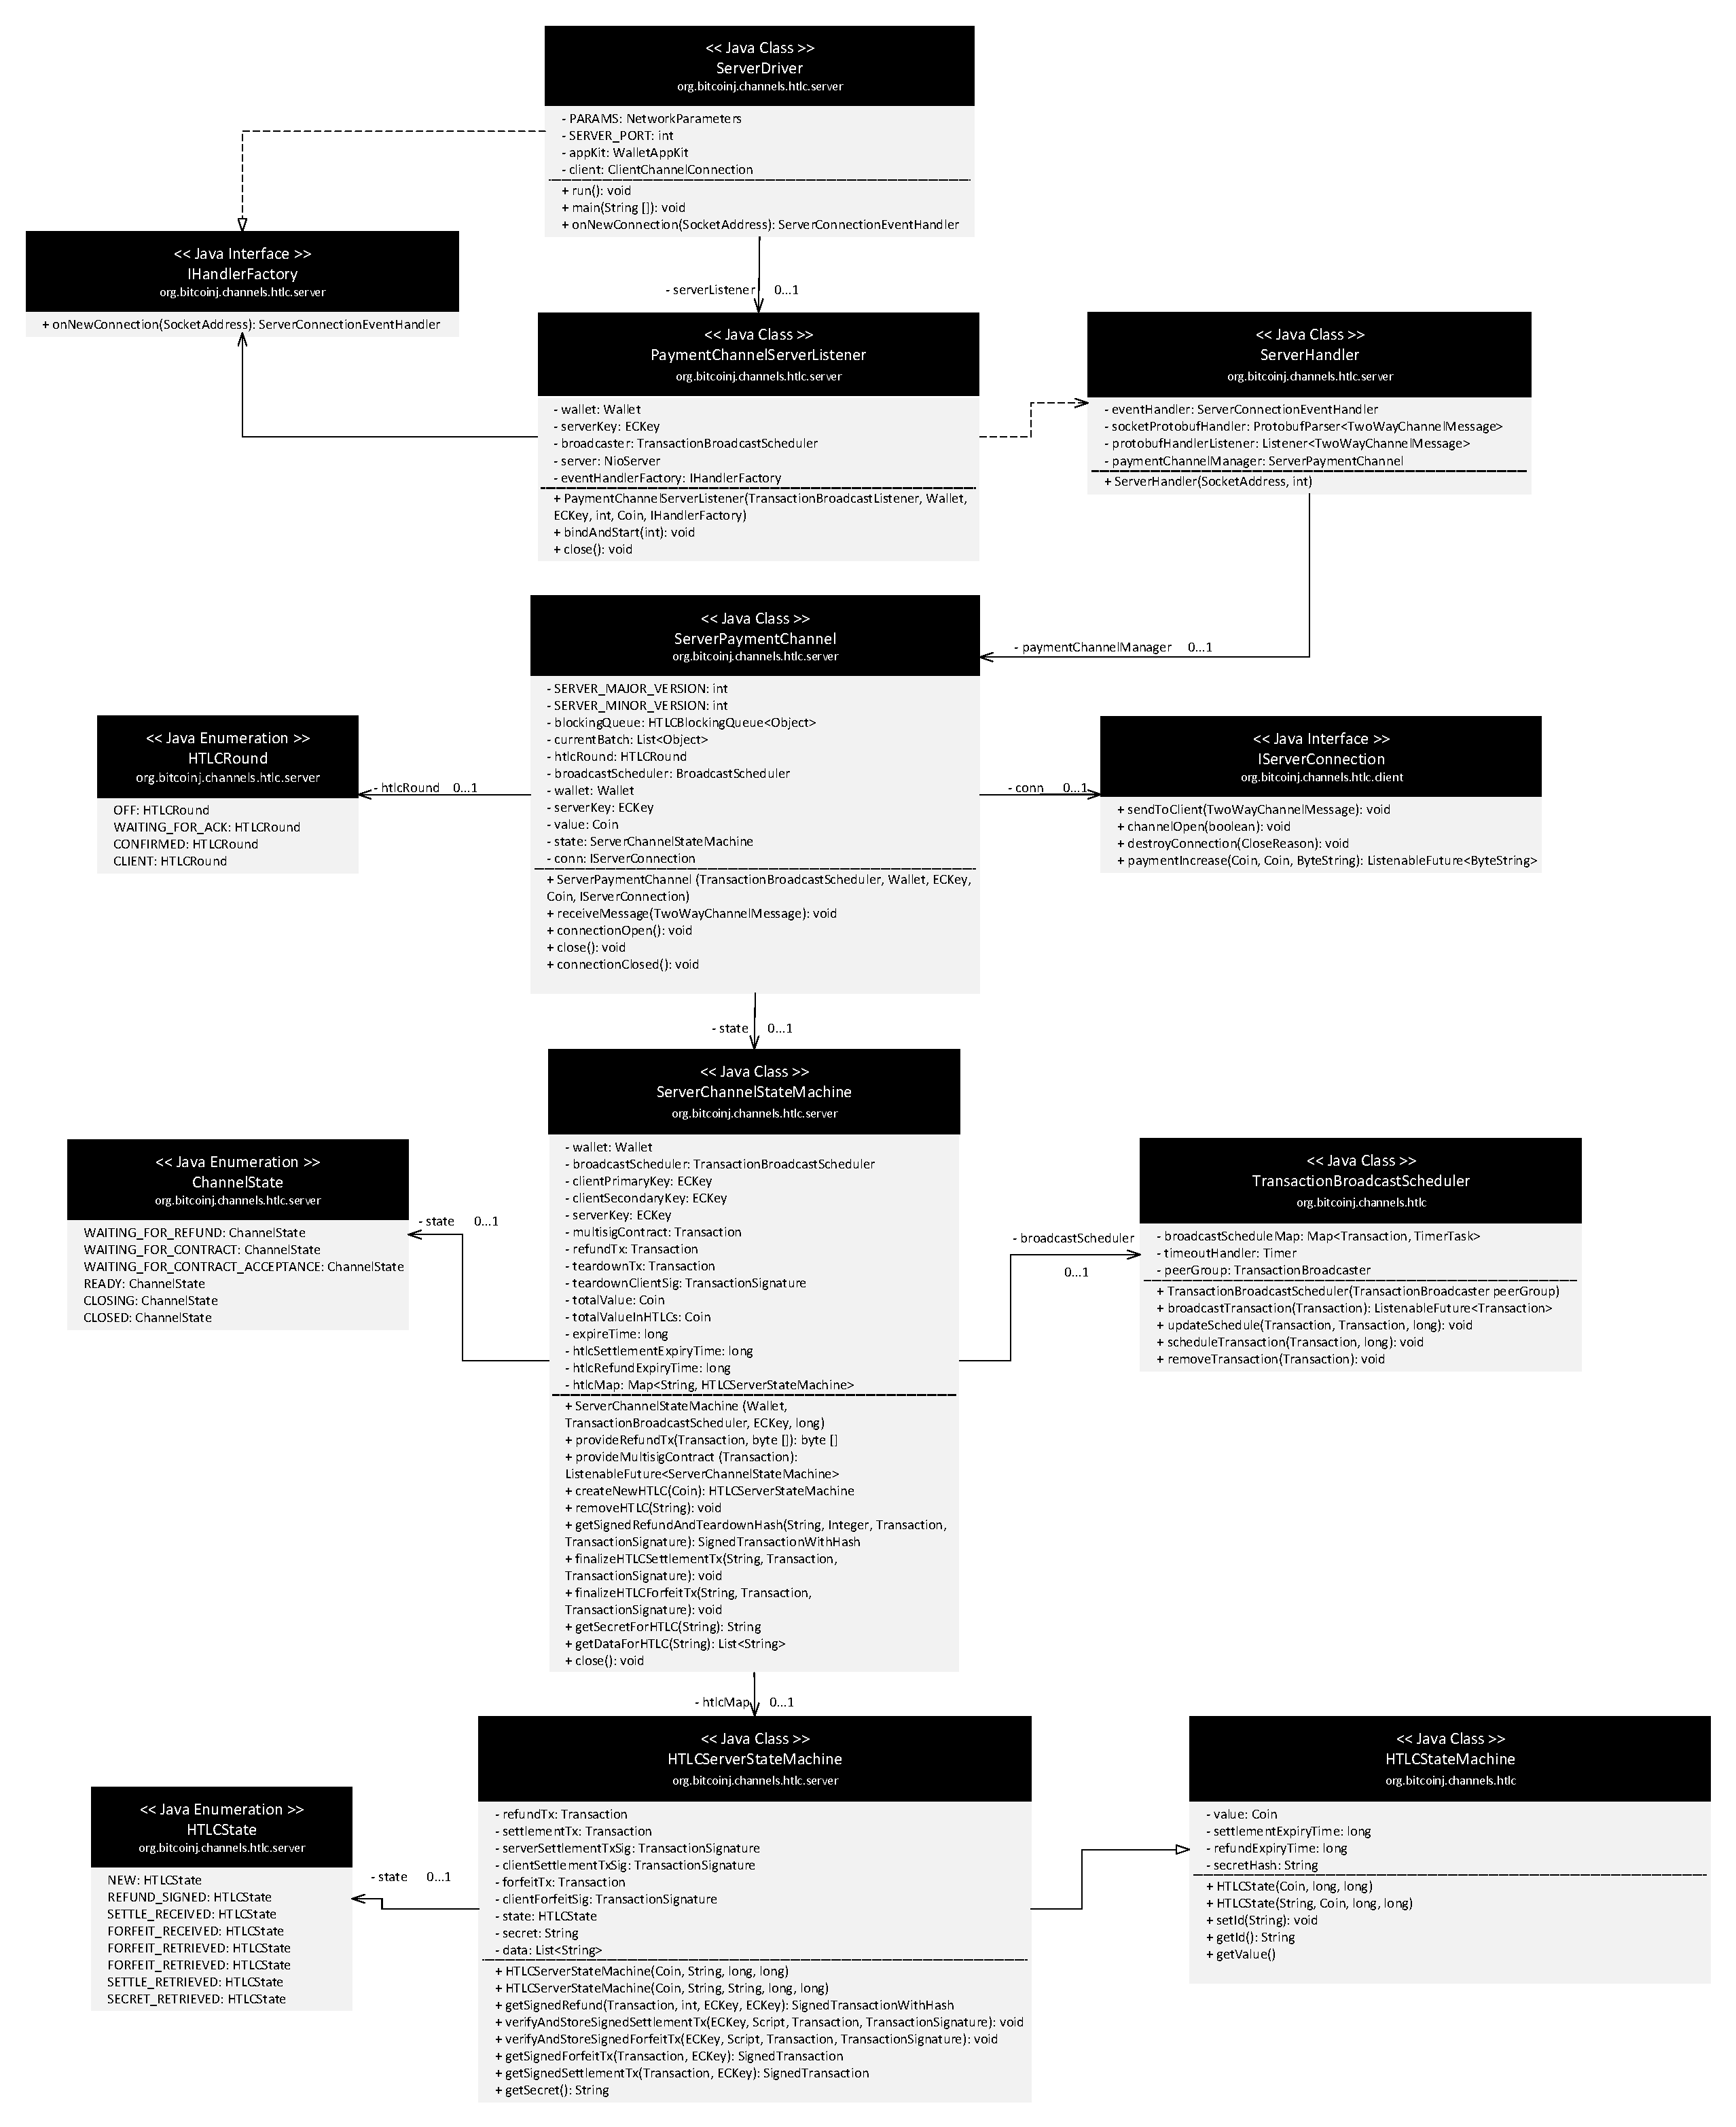
\includegraphics[width=1.2\textwidth]{figures/ServerUML}}
  \caption{UML class diagram of the Server component}
  \label{fig:serveruml}
\end{figure}

\begin{figure}[h]
  \centerline{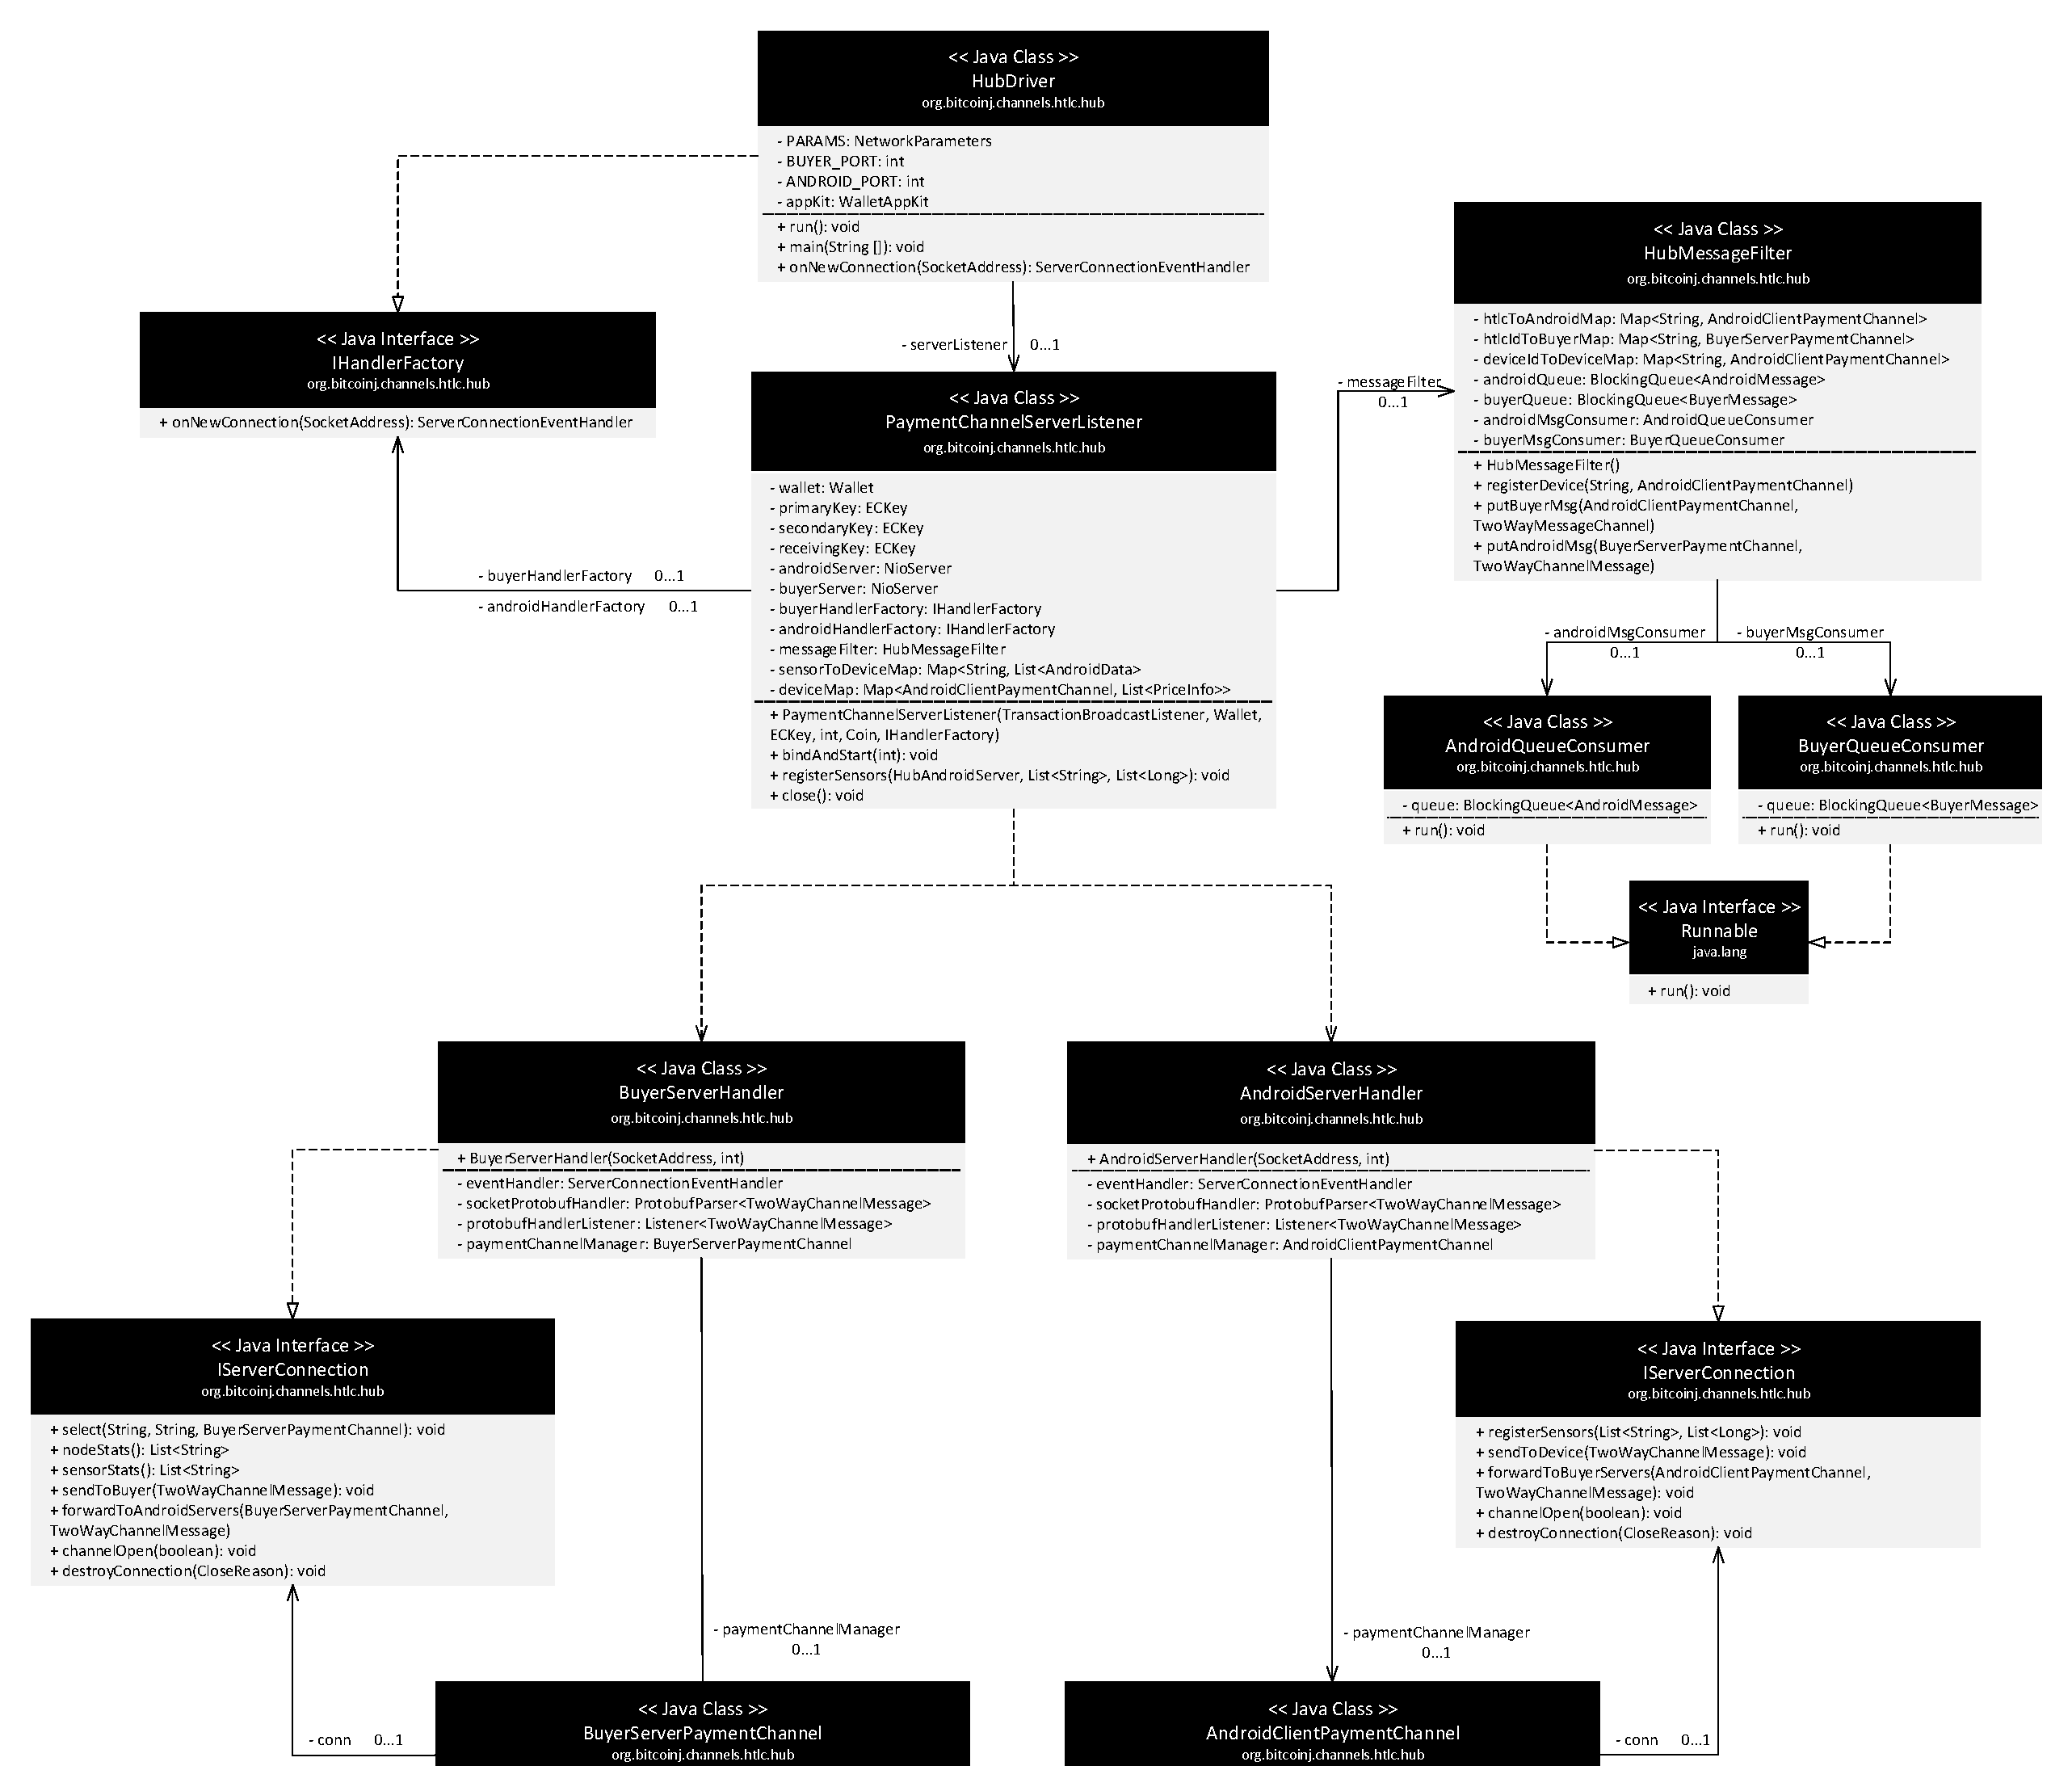
\includegraphics[width=1.25\textwidth]{figures/HubUML}}
  \caption{Hub class diagram of the first three layers.}
  \label{fig:hubuml}
\end{figure}

\end{document}